%\documentclass[11pt,a4paper]{article}
\documentclass[11pt
  , a4paper
  , article
  , oneside
%  , twoside
%  , draft
]{memoir}

\usepackage{control}
\usepackage[numbers]{natbib}

\begin{document}

\newcommand{\technumber}{
  RAON Control-Document Series\\
  Revision : v1.0,   Release : Jan. 02. 2015}
\title{\textbf{SNMP 이해 및 응답시간 테스트}}

\author{박미정\thanks{mijoy0909@ibs.re.kr} \\

  Rare Isotope Science Project\\
  Institute for Basic Science, Daejeon, South Korea
}
\date{\today}

\renewcommand{\maketitlehooka}{\begin{flushright}\textsf{\technumber}\end{flushright}}
%\renewcommand{\maketitlehookb}{\centering\textsf{\subtitle}}
%\renewcommand{\maketitlehookc}{C}
%\renewcommand{\maketitlehookd}{D}

\maketitle

\begin{abstract}
SNMP는 IP 네트워크에서 장치를 관리하기 위한 공식 인터넷 표준 프로토콜(Official Internet Standards Protocol)\citep{oisp}이다. 본 문서는 SNMP의 이해, SNMP를 이용한 장비 모니터링 결과 그리고 다양한 네트워크 환경에서 SNMP 버전 별 응답시간에 관한 테스트 결과에 대해 설명한다. 
\end{abstract}

\chapter{SNMP의 이해}
\section{SNMP란?}
SNMP(Simple Network Management Protocol)는 IP네트워크 상의 장치 및 장비들을 관리하고 모니터링하기 위한 인터넷 표준 프로토콜이다. SNMP는 Manager와 Agent로 구성되어있으며, Manager는 NMS(Network Management Stations)로 표현되기도 한다. Manager는 Agent에게 원하는 장비의 정보를 요청하며, 장비의 설정을 변경한다. Agent는 Manager가 요청한 장비의 정보를 제공하고, 시스템 충돌이나 재부팅 등의 장비에 영향을 미치거나 발생한 Event를 비동기적으로 알리기 위해 Trap 메세지를 보낸다. 이들의 관계는 그림 \ref{fig:relationship_m_a}\citep{essential_snmp}과 같다. 이는 원래 NMS와 Agent의 관계이지만 본 문서에서는 Manager와 Agent의 관계로 재구성하였다.
\begin{figure}[h!]
  \centering
  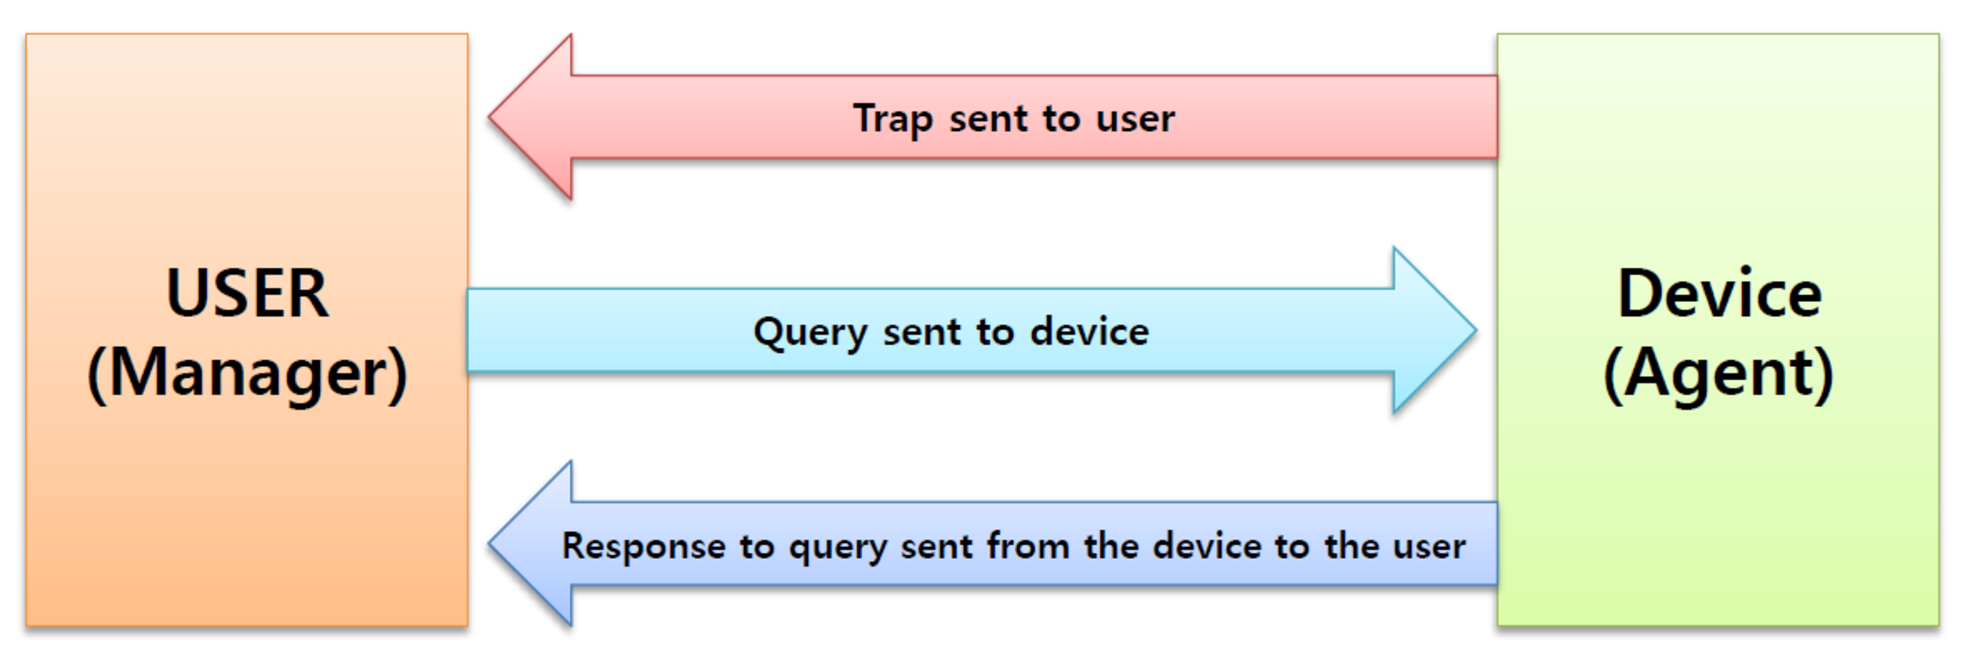
\includegraphics[width=0.65\textwidth]{./images/relationship_m_a.eps}
  \caption{Manager와 Agent의 관계}
  \label{fig:relationship_m_a}   
\end{figure}

\hfil\break
\hfil\break
\hfil\break
\hfil\break

SNMP는 v1/2c/3의 세 가지 버전이 있으며, 각 버전들은 인증과 암호화에 따른 차이점이 있다. SNMPv1/2c는 Community string에 의존한 문자열 일치로 사용자 인증을 하지만 암호화 하지 않는다. 반면 v3는 암호화 알고리즘(MD5, SHA, DES, AES)을 통한 인증과 암호화에 따라 noAuthNoPriv, authNoPriv, authPriv의 세 종류의 보안 레벨로 나뉜다. v3는 v1/2c에 비해 보안이 강화되지만 응답시간이 큰 단점이 있다. 자세한 SNMP 버전 별 차이점은 표 \ref{table:conparision}\citep{comparison}을 참조바란다.

\begin{table}[h!]
\begin{center}
\begin{tabular}{c|c|c|c}\hline
Version & Level & Authentication & Encryption \\ \hline
v1 & noAuthNoPriv & Community string & No \\ \hline
v2c & noAuthNoPriv & Community string & No \\ \hline
 & noAuthNoPriv & Username & No \\ \cline{2-4}
v3 & authNoPriv & MD5 or SHA & No \\ \cline{2-4}
 & authPriv & MD5 or SHA & DES or AES \\ \hline
\end{tabular}
\caption{SNMP 버전 별 차이점}
  \label{table:conparision} 
\end{center}
\end{table} 

\clearpage
\section{MIB(Management Information Base)}
SNMP를 지원하는 장치들은 MIB를 가지고 있으며, MIB는 관리되어야 할 장비에 대한 객체들을 계층구조로 모아 놓은 것으로 관리의 편의를 위해 그림 \ref{fig:oid_tree}와 같이 ROOT-Node에서 시작해 branch node와 leaf node로 이뤄진 Tree 구조를 가진다. 일반적인 TCP/IP관리정보는 MIB-2(RFC 1213)에 포함돼 있고, 특정 장비 관련 정보는 장비제조업체에서 제공한다. 

\begin{figure}[h!]
  \centering
  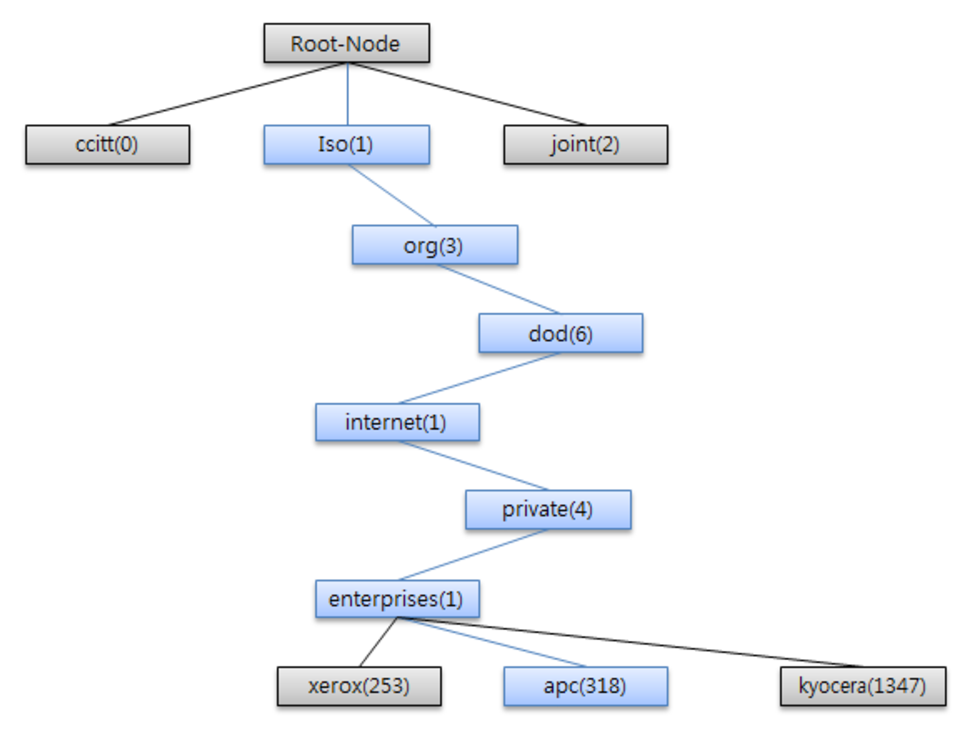
\includegraphics[width=0.65\textwidth]{./images/oid_tree.eps}
  \caption{MIB의 일반적 구조}
  \label{fig:oid_tree} 
\end{figure}

MIB내의 객체들은 고유의 식별자를 가지며 이를 OID(Object Identifiers)라 한다. 그림 \ref{fig:oid_tree}를 참고하면 APC사의 OID는 세 종류의 표기법에 따라 1.3.6.1.4.1.318, iso.org.dod.internet.\\private.enterprises.apc, iso(1).org(3).dod(6).internet(1).private(4).enterprises(1).apc(318)로 표현된다. OID는 그림 \ref{fig:ex_mib}과 같은 포맷을 가지며 이를 통해 객체의 데이터 타입, 필요 유무, 정의 그리고 접근권한(read-only, read-write, etc...)에 대해 알 수 있다. 

\begin{figure}[h!]
  \centering
  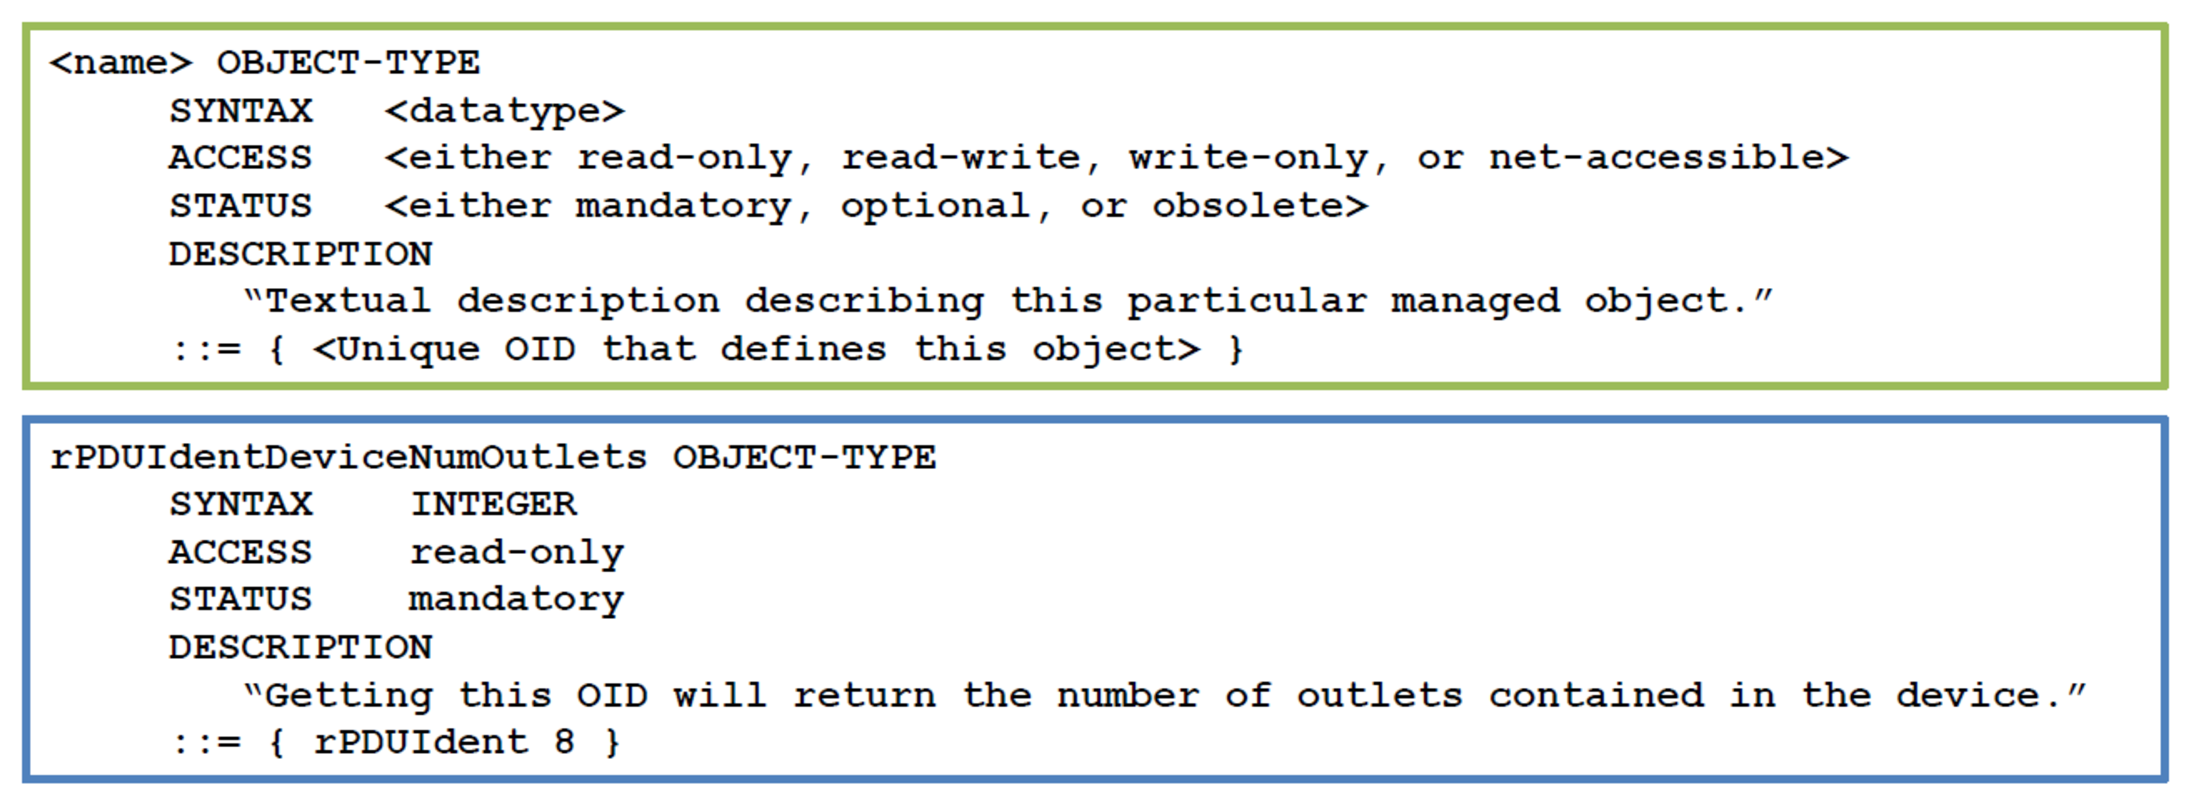
\includegraphics[width=0.8\textwidth]{./images/ex_mib.eps}
  \caption{OID 포맷의 예}
  \label{fig:ex_mib}   
\end{figure}


\subsection{1.2.1 MIB 파일 설정}
사용하고자 하는 장비의 MIB파일을 .snmp/snmp.conf파일(그림 \ref{fig:snmp_conf})에 추가하면 복잡한 OID번호 대신 MIB파일 내 객체 이름을 사용하여 장비의 정보를 요청할 수 있다.
snmp.conf 파일에 추가하기 앞서 MIB파일의 DEFINITIONS에 정의된 이름과 파일의 이름이 다를 경우 약간의 수정이 필요하다. 
\begin{figure}[h]
  \centering
  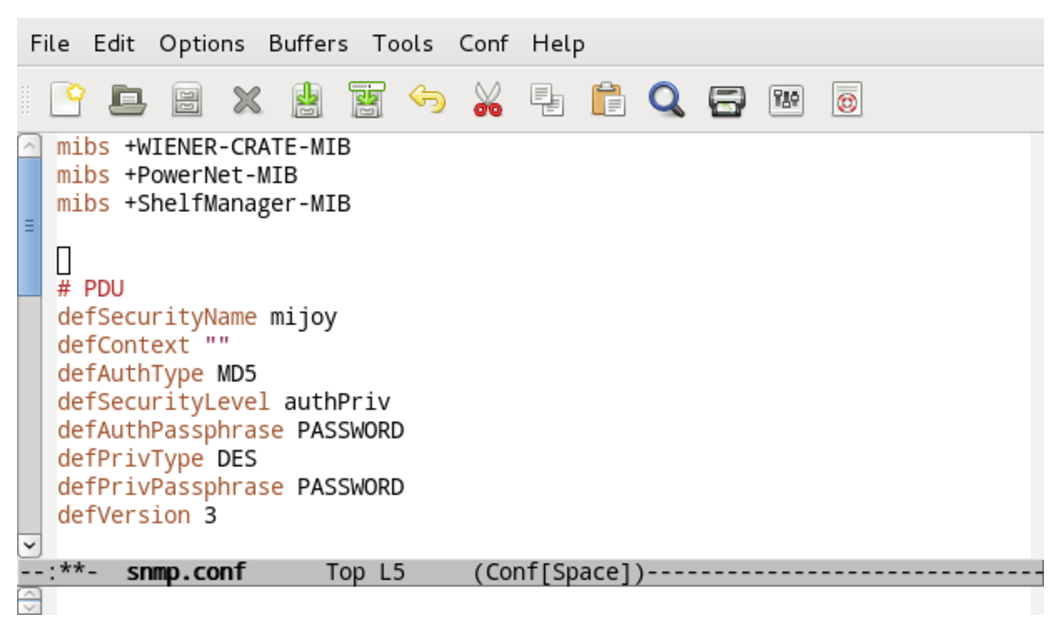
\includegraphics[width=0.79\textwidth]{./images/snmp_conf.eps}
  \caption{snmp.conf 파일}
  \label{fig:snmp_conf}   
\end{figure}

그림 \ref{fig:pdu_mib}는 APC사 PDU의 MIB파일의 일부분으로 다음과 같이 MIB파일의 DEFINITIONS ::= BEGIN에 파일의 이름(PowerNet-MIB)을 정의해주고, MIB파일명도 동일하게(PowerNet-MIB) 저장하면 된다. 이 과정을 거치면 OID번호가 아닌 객체 이름으로 장비의 정보를 읽고 쓸 수 있다. 


\begin{figure}[h]
  \centering
  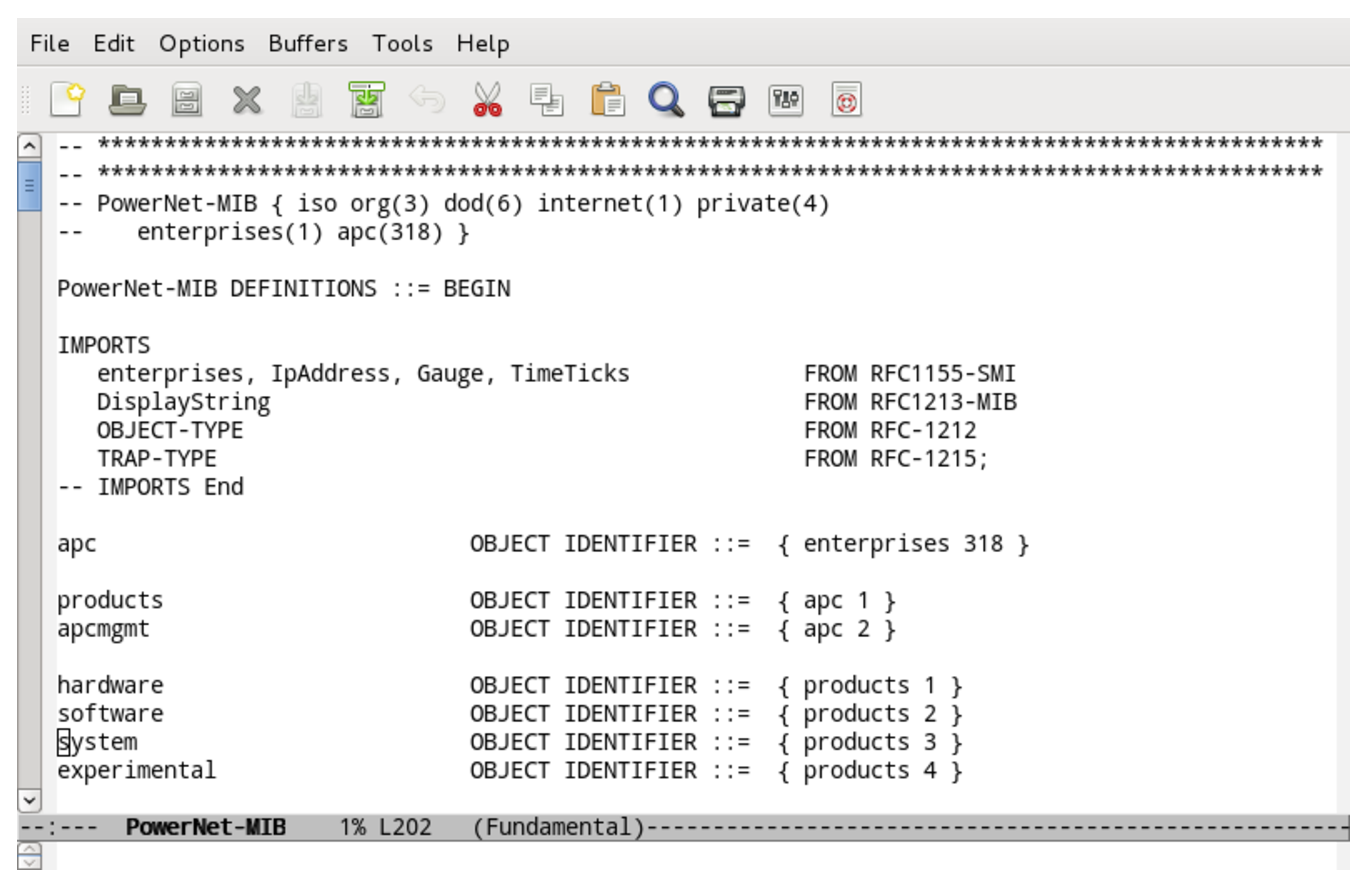
\includegraphics[width=0.79\textwidth]{./images/pdu_mib.eps}
  \caption{APC사 PDU의 MIB파일}
  \label{fig:pdu_mib}   
\end{figure}


\clearpage

\chapter{SNMP의 설치 및 사용}
\section{설치}
SNMP를 사용에 앞서 아래의 패키지를 설치해야 한다. 본 문서에서는 NET-SNMP\citep{net_snmp} v5.4.3을 사용하고 있다.
\begin{itemize}
\item NET-SNMP\footnote{* NET-SNMP는 http://www.net-snmp.org/download.html에서 다운받을 수 있다.}
\item snmp snmpd
\item snmp-mibs-downloader
\item libsnmp-dev libsnmp-base libsnmp-perl libsnmp15 
\end{itemize}


\section{SNMP 명령어와 사용}

\subsection{2.2.1 SNMPv3 설정}
SNMPv1/2c와 달리 SNMPv3는 사용에 따른 설정이 필요하다. 이는 앞서 설명 했듯 SNMPv3가 Username 및 보안레벨에 따른 암호화 알고리즘을 이용한 인증과 암호화를 하기 때문이다. 각 장비의 v3 관련 정보는 장비제조업체에서 제공하는 프로그램, 웹 페이지 및 시리얼 통신을 통해 설정 할 수 있다. localhost의 SNMPv3 설정은 다음과 같이 net-snmp의 snmpd로 가능하다. 이 때, 패스워드는 적어도 8자 이상이여야 한다.

\begin{lstlisting}[style=termstyle]
mijoy0909@mjpark:~$ su                                     
root@mjpark:~# service snmpd stop
Stopping network management services: snmpd snmptrapd.
root@mjpark:~# net-snmp-config --create-snmpv3-user
Enter a SNMPv3 user name to create: 
mijoy
Enter authentication pass-phrase: 
[password]
Enter encryption pass-phrase: 
  [press return to reuse the authentication pass-phrase]
[password]
adding the following line to /var/lib/snmp/snmpd.conf:
   createUser test MD5 "[password]" DES [password]
adding the following line to /usr/share/snmp/snmpd.conf:
   rwuser mijoy 
root@mjpark:~# service snmpd start
Starting network management services: snmpd.
\end{lstlisting}

snmpd를 설정은 /usr/share/snmp/snmpd.conf에서 아래와 같이 확인 가능하다. \footnote{* http://www.net-snmp.org/docs/README.snmpv3.html 참조 바람}

\begin{lstlisting}[style=termstyle]
rwuser mijoy
\end{lstlisting}


\subsection{2.2.2 SNMP 명령어}
SNMP를 이용해 장비의 정보를 요청하기 위해서는 SNMP명령어\footnote{* 자세한 설명은 http://www.net-snmp.org/wiki/index.php/Tutorials를 참조 바람}가 사용되며, 명령어는 SNMP의 버전에 따라 차이가 있다.

\begin{itemize}
\item get : Manager가 Agent에게 특정 정보를 요청 시 사용
\item getnext : get과 동일, 동일 계층의 다음 정보를 요청 시 사용
\item walk : get의 확장 형태, Tree구조에서 하위 트리들의 정보를 요청 시 사용
\item set : Manager가 특정 값을 변경 및 설정 시 사용
\item trap : Agent가 비동기적 사건을 Manager에게 알리기 위해 사용
\item etc...
\end{itemize}

\subsection{2.2.3 SNMP 명령어 사용 1 (walk, get)}
\subsubsection{- SNMPv1/2c}

\begin{lstlisting}[style=termstyle]
snmp(walk, get) -v (v1/2c) -c (Community String) (HostAddress) (OID) 
\end{lstlisting}

v1/2c의 Community string은 대부분 장비제조업체에서 public/privacy/admin으로 지정하지만, 사용자가 임의로 변경 가능하다. public은 read-only 권한을 privacy, admin은 read-write의 권한을 가지고 있다. 따라서 public을 이용하여 장비의 정보 값을 변경할 수 없다. v1/2c는 Community string을 사용한 사용자 인증 외에는 특별한 보안이 없어 보안에 취약하다는 것을 알 수 있다. 
\begin{lstlisting}[style=termstyle]
mijoy0909@mjpark:~$ snmpwalk -v 1 -c public localhost
RFC1213-MIB::sysDescr.0 = STRING: "Linux mjpark 3.2.0-4-amd64 #1 SMP Debian 3.2.63-2+deb7u2 x86_64"
RFC1213-MIB::sysObjectID.0 = OID: SNMPv2-SMI::enterprises.8072.3.2.10
RFC1213-MIB::sysUpTime.0 = Timeticks: (49138) 0:08:11.38
RFC1213-MIB::sysContact.0 = STRING: "Me <me@example.org>"
RFC1213-MIB::sysName.0 = STRING: "mjpark"
.
.
.
real	0m1.440s
user	0m0.224s
sys	0m0.084s
--------------------------------------------------------------------------------------------------
mijoy0909@mjpark:~$ snmpwalk -v 2c -c public localhost
RFC1213-MIB::sysDescr.0 = STRING: "Linux mjpark 3.2.0-4-amd64 #1 SMP Debian 3.2.63-2+deb7u2 x86_64"
RFC1213-MIB::sysObjectID.0 = OID: SNMPv2-SMI::enterprises.8072.3.2.10
RFC1213-MIB::sysUpTime.0 = Timeticks: (49138) 0:08:11.38
RFC1213-MIB::sysContact.0 = STRING: "Me <me@example.org>"
RFC1213-MIB::sysName.0 = STRING: "mjpark"
.
.
.
real	0m1.422s
user	0m0.220s
sys	0m0.096s
\end{lstlisting}

위의 결과는 snmpwalk명령어를 이용한 localhost의 정보 요청의 결과값이다. SNMPv1과 v2c는 결과의 차이가 없다.
\\
\subsubsection{- SNMPv3}
인증과 암호화에 따라서 v3명령어는 v1/2c와 차이를 보인다.
\begin{lstlisting}[style=termstyle]
snmp(walk, get) -v 3 -u (Username) -l {Security Level(noAuthNoPriv/authNoPriv/authPrive)} -a {Authentication Protocol(MD5/SHA)} -A (PASSWORD) -x {Privacy Protocol(DES/AES)} -X (PASSWORD) (HostAddress) (OID) 
\end{lstlisting}

SNMPv3의 snmpwalk를 이용해 요청한 localhost의 결과 값은 다음과 같다. v1/2c와 결과 값은 차이가 없지만 요청한 정보를 제공하는 응답시간에는 차이가 있음을 알 수 있다.
\begin{lstlisting}[style=termstyle]
mijoy0909@mjpark:~$ snmpwalk -v 3 -u mijoy -l authPriv -a MD5 -A  [PASSWORD]  -x DES -X  [PASSWORD]  localhost
RFC1213-MIB::sysDescr.0 = STRING: "Linux mjpark 3.2.0-4-amd64 #1 SMP Debian 3.2.63-2+deb7u2 x86_64"
RFC1213-MIB::sysObjectID.0 = OID: SNMPv2-SMI::enterprises.8072.3.2.10
RFC1213-MIB::sysUpTime.0 = Timeticks: (32928) 0:05:29.28
RFC1213-MIB::sysContact.0 = STRING: "Me <me@example.org>"
RFC1213-MIB::sysName.0 = STRING: "mjpark"
.
.
.
real	0m1.773s
user	0m0.340s
sys	0m0.124s
\end{lstlisting}

장비의 모든 정보만 요청하는 snmpwalk와 달리 snmpget을 이용하면 아래와 같이 필요한 정보의 값을 선택적으로 읽을 수 있다.
\begin{lstlisting}[style=termstyle]
mijoy0909@mjpark:~$ snmpget -v 2c -c public localhost RFC1213-MIB::sysName.0
RFC1213-MIB::sysName.0 = STRING: "mjpark"
.
.
mijoy0909@mjpark:~$ snmpget -v 1 -c public localhost RFC1213-MIB::sysName.0 RFC1213-MIB::sysObjectID.0
RFC1213-MIB::sysName.0 = STRING: "mjpark"
RFC1213-MIB::sysObjectID.0 = OID: SNMPv2-SMI::enterprises.8072.3.2.10
\end{lstlisting}

\subsection{2.2.4 SNMP 명령어 사용 2 (set)}

snmpwalk, get과 달리 set은 장비의 정보를 설정 및 변경하고자 할 때 사용된다. 이 때, 아래와 같이 객체가 가진 데이터 타입에 따른 옵션이 필요하다.

\begin{lstlisting}[style=termstyle]
 i: INTEGER 
 u: unsigned INTEGER 
 t: TIMETICKS
 a: IPADDRESS
 o: OBJID
 s: STRING
 x: HEX STRING
 d: DECIMAL STRING
 U: unsigned int64
 I: signed int64
 F: float
 D: double
\end{lstlisting}

\subsubsection{- SNMPv1/2c}

\begin{lstlisting}[style=termstyle]
mijoy0909@mjpark:~$ snmpset -v (v1/2c) -c (Community String) (HostAddress) (OID) (datatypes) (value)
\end{lstlisting}

\subsubsection{- SNMPv3}

\begin{lstlisting}[style=termstyle]
mijoy0909@mjpark:~$ snmpset -v 3 -u (Username) -l {Security Level(noAuthNoPriv/authNoPriv/authPrive)} -a {Authentication Protocol(MD5/SHA)} -A (PASSWORD) -x {Privacy Protocol(DES/AES)} -X (PASSWORD) (HostAddress) (OID) (datatypes) (value)
\end{lstlisting}

다음은 APC사의 Power Distribution Unit의 정보를 v3를 이용하여 Outlet8번의 전원을 설정한 결과이다. snmpset도 snmpget과 마찬가지로 선택적으로 값을 쓸 수 있다.

\begin{lstlisting}[style=termstyle]
snmpset -v 3 -u mijoy -l authPriv -a MD5 -A [PASSWORD] -x DES -X [PASSWORD] 10.1.5.142 sPDUOutletCtl.8 i 2
PowerNet-MIB::sPDUOutletCtl.8 = INTEGER: outletOff(2)
.
.
snmpset -v 3 -u mijoy -l authPriv -a MD5 -A [PASSWORD] -x DES -X [PASSWORD] 10.1.5.142 sPDUOutletCtl.7 i 1 sPDUOutletCtl.8 i 1
PowerNet-MIB::sPDUOutletCtl.7 = INTEGER: outletOn(1)
PowerNet-MIB::sPDUOutletCtl.8 = INTEGER: outletOn(1)
\end{lstlisting}

추가적으로 SNMPv1/2c와 달리 v3의 명령어가 긴 문제를 해결하기 위해서 그림 \ref{fig:snmp_conf}와 같이 snmp.conf파일에 미리 v3에 대한 보안레벨과 암호화 알고리즘을 설정하고 패스워드정보를 저장해둔다면 아래와 같이 간단하게 SNMPv3를 사용할 수 있다.\footnote{* 여러가지 장비의 정보를 설정한 후 장비의 정보를 요청한 결과 첫 번째로 저장된 설정에서만 간편하게 SNMPv3 사용이 가능하였다. 이는 추가적인 확인이 필요한데, 만약 첫 번째로 저장된 설정에서만 가능하다면 v3를 사용하고자 하는 장비의 보안레벨, 암호화 프로토콜, 그리고 패스워드를 통일하는 작업이 필요 할 것 같다.}

\begin{lstlisting}[style=termstyle]
mijoy0909@mjpark:~$ snmpget 10.1.5.142 sPDUIdentModelNumber
PowerNet-MIB::sPDUIdentModelNumber.0 = STRING: "AP7921"
\end{lstlisting}

이 외의 SNMP의 추가적인 옵션은 snmp(walk, get, set, trap...) -h를 이용해 알 수 있다.

\clearpage
\section{SNMP를 이용한 장비 모니터링}
본 문서에 사용된 시스템, 소프트웨어 및 하드웨어의 정보 그리고 장비제조업체에서 지원하는 SNMP버전\footnote{*본 문서에서 Read는 모니터링, Write는 제어라 칭한다.}은 다음과 같다.
\subsection{2.3.1 시스템 및 소프트웨어}
\begin{itemize}
\item Debian Linux 7 Wheezy
\item NET-SNMP v5.4.3
\item GNU Bash script-CLI(Command-line Interface) 
\end{itemize}

\subsection{2.3.2 하드웨어 및 SNMP지원버전\ref{table:used_version}}

\begin{table}[h]
\begin{center}
\begin{tabular}{c|c}\hline
Device Name & Supported Versions \\ \hline
Printer(Xerox, Kyocera) & v1* (R) \\ \hline
WIENER VME CRATE & v1/2c* (R/W) \\ \hline
ELMA VME CRATE & v3* (R) \\ \hline
APC PDU 7921 & v1/2c/3* (R/W) \\ \hline
\end{tabular}
\caption{모니터링에 사용된 장비와 장비 별 지원하는 SNMP 버전}
{(R: Read, W: Write / *: 모니터링에 사용된 버전)}
  \label{table:used_version}  
\end{center}
\end{table} 

\clearpage
\subsection{2.3.3 모니터링 결과}
\subsubsection{2.3.3.1 프린터(Xerox \& Kyocera)}

Xerox사와 Kyocera사의 프린터들에 설정되어 있는 SNMP Agent의 기본 설정을 사용하여 프린터의 현재 상태, 용지의 종류와 양, 잉크의 잔여량 등의 정보를 SNMPv1로 모니터링한 결과이다. 

\begin{lstlisting}[style=termstyle, caption=Xerox \& Kyocera사 Printer 모니터링 결과]]
mijoy0909@mjpark:~/users/mijoy0909$ ./snmptest.sh 
 
Mon Nov 17 10:35:17 KST 2014
 
++++++++++++++++ Printer Status ++++++++++++++++
- 182 Printer              -, "Printing..." "" ""
- 184 Printer              -, "Sleeping " " "
 
++++++++ 182 Printer Paper Current Level ++++++++
- Tray1                    -, 25.000%
- Tray2                    -, 0%
- Tray3                    -, 75.000%
- Tray4                    -, 75.000%
- Tray5                    -, 0%
 
++++++++ 182 Printer Paper Current size ++++++++
- Tray1                    -, A4
- Tray2                    -, A4
- Tray3                    -, A4
- Tray4                    -, A3
- Tray5                    -, -
 
++++++++ 184 Printer Paper Current Level ++++++++
- MP Tray                  -, 0%
- Tray1                    -, 50.000%
- Tray2                    -, 0%
- Tray3                    -, 50.000%
- Tray4                    -, 50.000%
 
++++++++ 184 Printer Paper Current size ++++++++
- MP Tray                  -, A4
- Tray1                    -, A4
- Tray2                    -, -
- Tray3                    -, A3
- Tray4                    -, A3
 
++++++++ 182 Printer Toner Current Level ++++++++
- black                    -, 97.000%
- yellow                   -, 6.000%
- magenta                  -, 9.000%
- cyan                     -, 40.000%
 
++++++++ 184 Printer Toner Current Level ++++++++
- black                    -, 73.000%
 
+++++++++ 182 Printer Printed Page(s) ++++++++++
- total                    -, 477124
 
+++++++++ 184 Printer Printed Page(s) ++++++++++
- total                    -, 86618
\end{lstlisting}


\subsubsection{2.3.3.2 VMEbus Crate(Elma \& Wiener)}
VMEbus Crate(그림 \ref{fig:elmawiener})들은 가속기를 제어하는데 있어 중요한 장비들이며, 가속기 시설의 특성상 즉각적인 접근이 불가능한 지역에 설치되는 경우가 많다. 이러한 이유로 다른 장비들과 다르게 모니터링뿐만 아니라 제어도 가능해야 하며, 따라서 신호의 보안에도 신경을 써야한다. 

\begin{figure}[h]
  \centering
  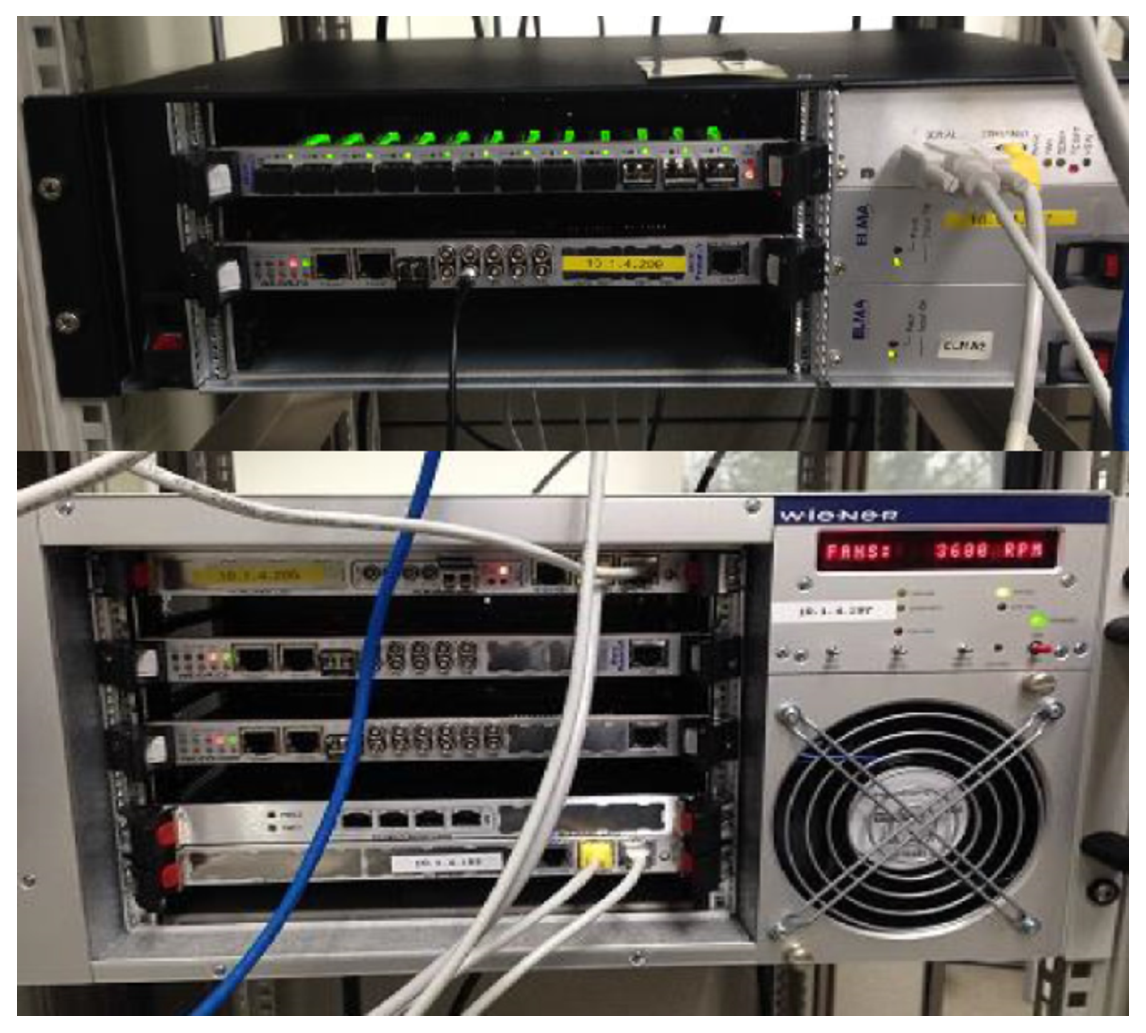
\includegraphics[width=0.7\textwidth]{./images/elmawiener.eps}
  \caption{Elma, Wiener Crate (위 : Elma, 아래: Wiener)}
  \label{fig:elmawiener}   
\end{figure}

\vspace{2mm}

본 문서에서 Elma사의 Crate는 SNMPv3로 Crate 상태, 온도 등을 모니터링했고, Wiener사의 Crate는 현재 지원하는 SNMPv2c로 Crate의 상태, 팬 스피드, 온도 등에 대한 모니터링과 스위치의 동작 및 팬 스피드를 제어했다. 

\clearpage

- Elma Crate
\begin{lstlisting}[style=termstyle, caption=ELMA Crate 모니터링 결과]]
mijoy0909@mjpark:~/users/mijoy0909$ ./elma_test1.sh

- Voltage
==================================================
   #         Name          Value          State
==================================================
   1     "+3.3V"          3.290 V          OK
   2       "+5V"          4.980 V          OK
   3      "+12V"         11.960 V          OK
   4      "-12V"    2147483.647 V          OK
==================================================

- Temp
==================================================
   #         Name          Value          State
==================================================
   1       "Temp 1"       37 deg C         OK
   2       "Temp 2"       27 deg C         OK
   3       "Temp 3"       24 deg C         OK
==================================================

- Fan
==================================================
   #         Name          Value          State
==================================================
   1        "Fan 1"       3400 RPM         OK
   2        "Fan 2"       3400 RPM         OK
   3        "Fan 3"       3400 RPM         OK
   4        "Fan 4"       3400 RPM         OK
   5        "Fan 5"       3500 RPM         OK
   6        "Fan 6"       3400 RPM         OK
==================================================
\end{lstlisting}

\clearpage
- Wiener Crate
\begin{lstlisting}[style=termstyle, caption=Wiener Crate 모니터링 및 제어결과]]
***************************************
*               OPTIONS               *
***************************************
  [s] Status                           
  [1] Main Switch ON/OFF               
  [2] Change Fan Speed (1200~3600 RPM) 
  [q] Exit                             
  [0] Help                             
***************************************
-> Please enter your choice : 2

- Main Switch : ON
- Fan Speed : 3500 RPM
- Temperature Sensors1 : 25 deg C
- Temperature Sensors2 : 22 deg C

- Voltage
========================================
 Name        Value          State
========================================
  U0         3.33 V           On
  U1         5.01 V           On
  U2        12.06 V           On
  U3       -12.24 V           On
========================================

Enter Fan Speed (0~3600 RPM) : 
3600
INTEGER: 3600 RPM

- Main Switch : ON
- Fan Speed : 3600 RPM
- Temperature Sensors1 : 25 deg C
- Temperature Sensors2 : 22 deg C
\end{lstlisting}

\clearpage
\subsubsection{2.3.3.3 Power Distribution Unit}
VMEbus Crate와 마찬가지로 Power supply 또한 모니터링과 제어가 가능해야 한다. 모든 버전의 SNMP를 지원하는 APC사의 Power Distribution Unit (PDU) 7921(그림 \ref{fig:apc_pdu})을 이용하여, SNMPv3에서 모니터링과 제어에 필요한 여러 설정을 테스트 해 보았다. 아래는 SNMPv3를 통해 APC PDU의 장비의 상태, 사용전력, 부하된 전류량 등을 모니터링하고 장비에서 지원하는 다양한 옵션으로 각각의 Power Outlet을 제어한 결과이다.
\begin{figure}[h]
  \centering
  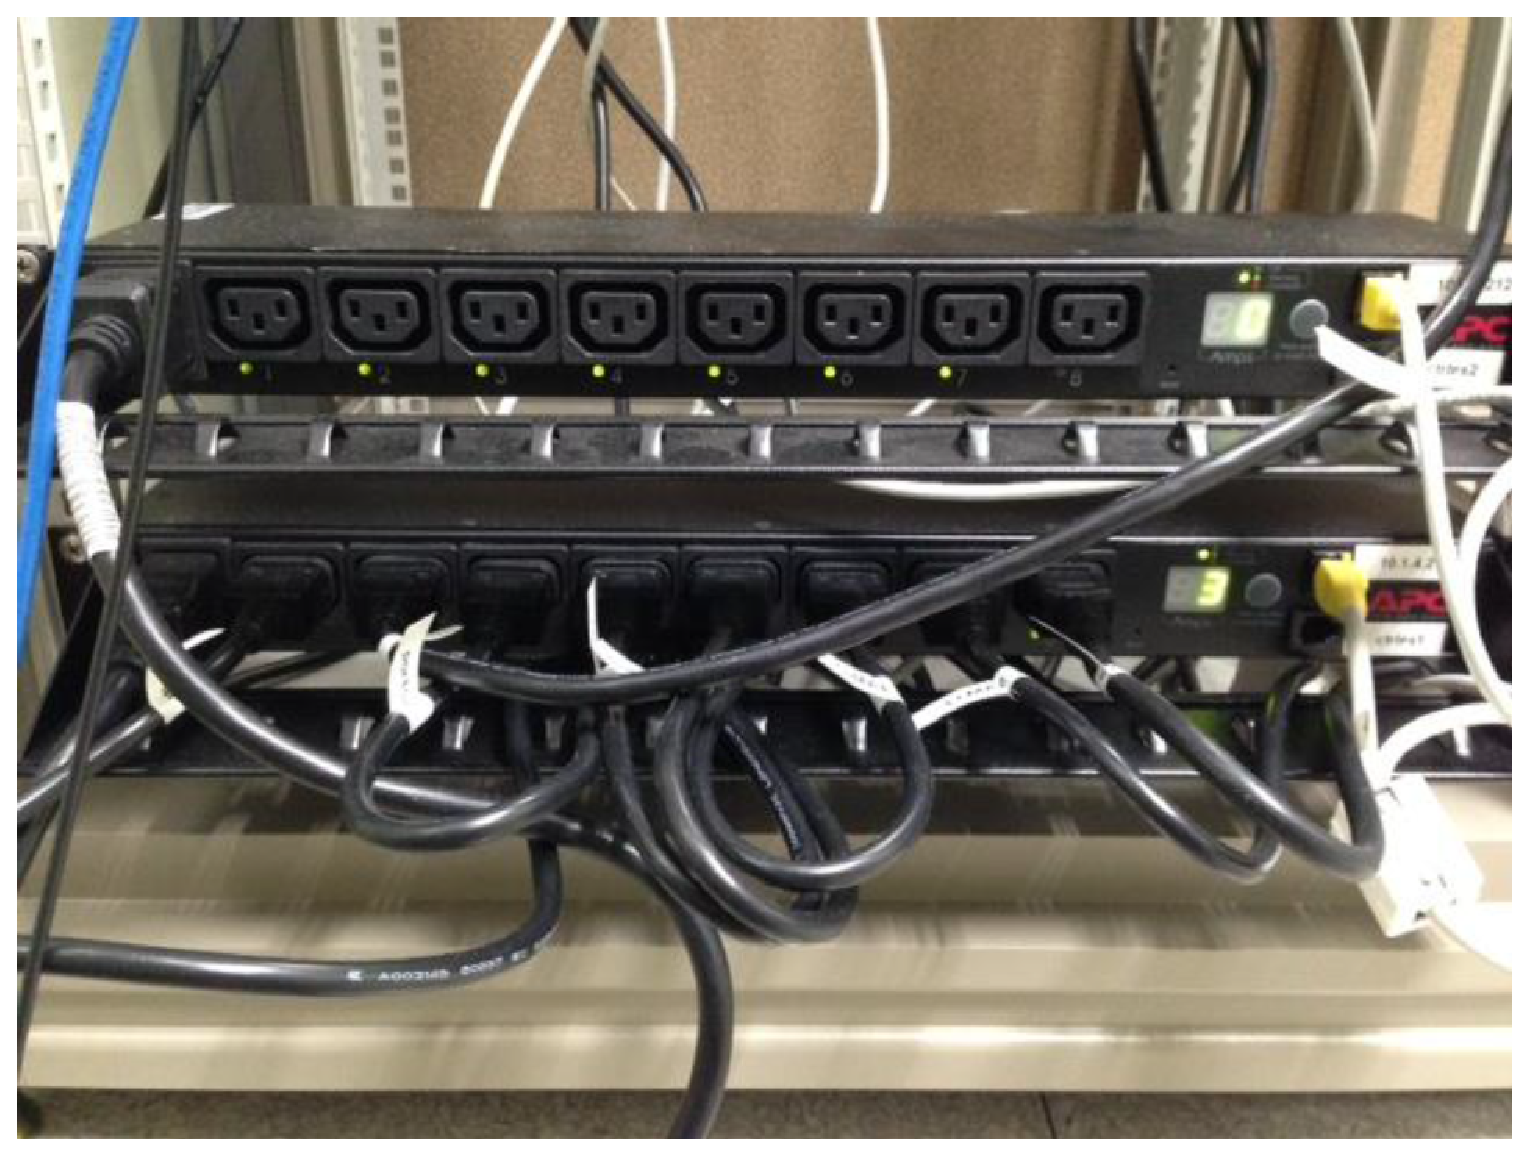
\includegraphics[width=0.6\textwidth]{./images/apc_pdu.eps}
  \caption{APC PDU}
  \label{fig:apc_pdu}   
\end{figure}

\begin{lstlisting}[style=termstyle, caption=APC PDU 모니터링 및 제어결과]]
mijoy0909@mjpark:~/users/mijoy0909$ ./powernet_test8.sh

*****************************
*          OPTIONS          *
*****************************
  [s] Status                 
  [1] ON                     
  [2] OFF                    
  [3] Reboot                 
  [4] On with delay          
  [5] Off with delay         
  [6] Reboot with delay      
  [q] Exit                   
  [0] Help                   
*****************************
-> Please enter your choice : 2

------------------------------------------------------------
 PowerWatts                      , 220
 Load Status                     , 1.0 Amps

   #       Name       Status      Control Outlet Command
============================================================
   1     "Outlet 1"      On              immediateOn
   2     "Outlet 2"      On              immediateOn
   3     "Outlet 3"      On              immediateOn
   4     "Outlet 4"      On              immediateOn
   5     "Outlet 5"      On              immediateOn
   6     "Outlet 6"      On              immediateOn
   7     "Outlet 7"      On              immediateOn
   8     "Outlet 8"      On              immediateOn
============================================================
------------------------------------------------------------
  [s] Status                 
  [1] Outlet1                
  [2] Outlet2                
  [3] Outlet3                
  [4] Outlet4                
  [5] Outlet5                
  [6] Outlet6                
  [7] Outlet7                
  [8] Outlet8                
  [b] Back                   
  [q] Exit                   
  [0] Help                   
-> Select outlet: 8
-> Are you sure? [y/n]y
outletOff

------------------------------------------------------------
 PowerWatts                      , 220
 Load Status                     , 1.0 Amps

   #       Name       Status      Control Outlet Command
============================================================
   1     "Outlet 1"      On              immediateOn
   2     "Outlet 2"      On              immediateOn
   3     "Outlet 3"      On              immediateOn
   4     "Outlet 4"      On              immediateOn
   5     "Outlet 5"      On              immediateOn
   6     "Outlet 6"      On              immediateOn
   7     "Outlet 7"      On              immediateOn
   8     "Outlet 8"     Off             immediateOff
============================================================
------------------------------------------------------------
\end{lstlisting}


\clearpage

\chapter{SNMP 버전 별 응답시간 실험}
가속기 제어 시스템에서 시설의 복잡성과 장비의 다양성, 그리고 안전한 장비 접근성을 만족하며, 동시에 장비의 안정된 응답시간을 만족시키는 설치 위치를 선정하는 것은 어렵기 때문에 장비의 응답시간을 고려하여 제어 네트워크 토폴로지 설계 및 네트워크 보안에 따른 SNMP의 응답시간 최적화 설계가 필요하다. 따라서 실험 당시 SNMP의 모든 버전(v1/2c/3)을 지원하는 장비인 APC PDU 7921을 사용하여 모니터링 및 제어에 걸리는 SNMP 버전 별 응답시간에 대한 실험을 진행했다.

\begin{table}[h!]
\begin{center}
\begin{tabular}{c|c|c|c|c}\hline
 & v1 & v2c & v3(R) & v3(W) \\ \hline
mean & 2.863 & 2.852 & 4.101 & 4.138 \\ \hline
sample deviation & 0.867 & 0.840 & 0.814 & 0.864 \\ \hline
\end{tabular}
\caption{SNMP 버전에 따른 응답시간(wall-clock time response)의 차이 (단위: ms)}
  \label{table:test}  
\end{center}
\end{table}
표 \ref{table:test}은 암호화 및 복호화에 걸리는 시간, 케이블 딜레이, 하드웨어 자체의 속도 및 사용된 Linux OS에 대한 응답시간 차이가 동일하다는 가정하에 장비의 정보를 요청 시 SNMP 버전 별 응답시간을 측정한 결과이다. 이 결과로 SNMPv1/2c는 서로 비교할 수 없는 오차 범위에 있으며, v3는 모니터링과 제어에서 타 버전에 비해 1.5배 정도의 시간이 더 소모됨을 확인 할 수 있다.

\section{실험 목적}
앞서 언급했듯이 장비의 응답시간은 제어 네트워크에서 중요하다. 가속기 제어 네트워크 토폴로지 설계에 필요한 물리적인 구성요소는 Layer 2 스위치와 UTP 케이블의 길이이므로 이러한 요소들이 토폴로지 내에서 가능하고, 이상적인 장비의 응답시간과 구성요소들 간의 상관관계를 측정하는 것이 필요하다. 이렇게 측정된 결과들은 네트워크 토폴로지 설계 및 장비의 최적화된 설치위치 선정에 도움이 될 것이다.

\section{실험 방법}
본 실험에서는 프로그램이 수행되는 시간을 측정하는 리눅스의 time 명령어를 이용하여 SNMP명령어를 1000번 수행한 시간을 응답시간으로 측정하였다. time 명령어는 아래와 같이 세 가지 형태의 시간 측정 결과를 나타낸다\citep{time_command}. 
\begin{itemize}
\item real : 실제로 걸린 시간
\item user : 커널이 사용한 시간을 제외한 CPU에서 소비된 시간
\item sys : 실제로 할애한 커널 시간
\end{itemize}
이를 참조하면 user+sys의 시간은 실제로 작업에 할애된 시간이며, real-(user+sys)의 시간은 다른 프로세서 처리에 할당된 시간이다. 따라서 본 문서의 실험에서는 실제 작업 시간인 user+sys시간을 사용한다. 이는 Layer 2 스위치 간의 내부 시간 차이와 케이블을 제작 시 발생하는 길이의 오차 등에서 발생하는 시간이 포함된 것이다. UTP케이블이 물리적으로 신호를 안정적으로 전달할 수 있는 최대 길이가 100m이기 때문에 본 실험에는 1m, 10m, 20m, 30m, 40m, 50m, 100m 길이의 CAT6 LAN 케이블을 사용하였다.

\subsection{3.2.1 시스템 및 소프트웨어}
실험에 사용된 시스템, 소프트웨어, 그리고 하드웨어는 아래와 같다.

\begin{itemize}
\item Debian Linux 7 Wheezy
\item NET-SNMP v5.4.3
\item R v2.15.1
\item GNU Bash Script-CLI(Command-line Interface) 
\item Switch(BROCADE ICX6430)
\item Power Distribution Unit(APC PDU 7921)
\end{itemize}

\subsection{3.2.2 Bash Script 구성}
본 문서의 SNMPv1/2c/3의 응답시간 측정에는 GNU Bash를 이용하여 만든 Script를 사용한다. 이 Script는 지정한 시간동안 시스템을 멈추는 리눅스 sleep 명령어를 사용해 시스템을 1초 멈추는 조건과 sleep을 사용하지 않는 조건으로 snmpget, set 명령어를 사용해 장비의 정보를 1000번 요청하고 응답받는다. 이 과정에 걸린 시간을 time 명령어로 측정하고, CLI로 total count, mean, sample deviation, standard deviation의 측정 결과를 보인다.

\begin{lstlisting}[style=termstyle, caption=GNU Bash script를 통한 CLI]
mijoy0909@mjpark:~/speedtest$ ./speedtest.sh 

**********************************
*               OPTIONS          *
**********************************
  [1] SNMP Speed Test             
  [2] File Merge                  
  [3] R(Linear)                   
  [4] R(Histogram)                
----------------------------------
----------------------------------
  [5] Edit R(linear)              
  [6] Edit R(histogram)           
----------------------------------
----------------------------------
  [q] Exit                        
  [0] Help                        
**********************************
-> Select sub option: 1

****************************************
*              SUB OPTIONS             *
****************************************
  [1] SNMP v1        / sleep x          
  [2] SNMP v1        / sleep 1          
  [3] SNMP v2c       / sleep x          
  [4] SNMP v2c       / sleep 1          
  [5] SNMP v3(read)  / sleep x          
  [6] SNMP v3(read)  / sleep 1          
  [7] SNMP v3(write) / sleep x          
  [8] SNMP v3(write) / sleep 1          
  [b] Back                              
  [q] Exit                              
  [0] Help                              
***************************************
-> Select sub option: 1

Enter name you wish to save [ex.example] :S1V1SXC1
/home/mijoy0909/speedtest
outletOn
outletOn
.
outletOn
-----------------------------------------------
<real>

Total count        :       1000
Mean               : 0.09147000
Sample Deviation   : 0.00503631
Standard Deviation : 0.00503380

-----------------------------------------------
<user>

Total count        :       1000
Mean               : 0.06384000
Sample Deviation   : 0.00590672
Standard Deviation : 0.00590376

-----------------------------------------------
<sys>

Total count        :       1000
Mean               : 0.00061000
Sample Deviation   : 0.00247670
Standard Deviation : 0.00247546

***********************************************

Mean(user+sys)             : 0.03222500
Sample Deviation(user+sys) : 0.00640495

***********************************************
-----------------------------------------------
\end{lstlisting}

\subsection{3.2.3 실험 배치도 및 방법}
그림 \ref{fig:switch}은 스위치 5개를 연결 했을 때의 실험 배치도이다. 예를 들어 길이가 1m인 케이블을 이용한 응답시간 측정 시에 컴퓨터, PDU, 스위치를 1m의 네트워크 케이블로 연결한 후 Script를 실행하여 응답시간을 측정한다. 점차 스위치의 개수를 증가시키면서 테스트를 진행한다. 이 때, 컴퓨터는 첫 번째 스위치 계속해 연결되어있고, 스위치의 개수를 5개까지 추가하면서 마지막 스위치에 PDU를 연결한다. 다른 길이의 케이블도 각각 위의 과정을 수행한다. 

\begin{figure}[!htb]
  \centering
  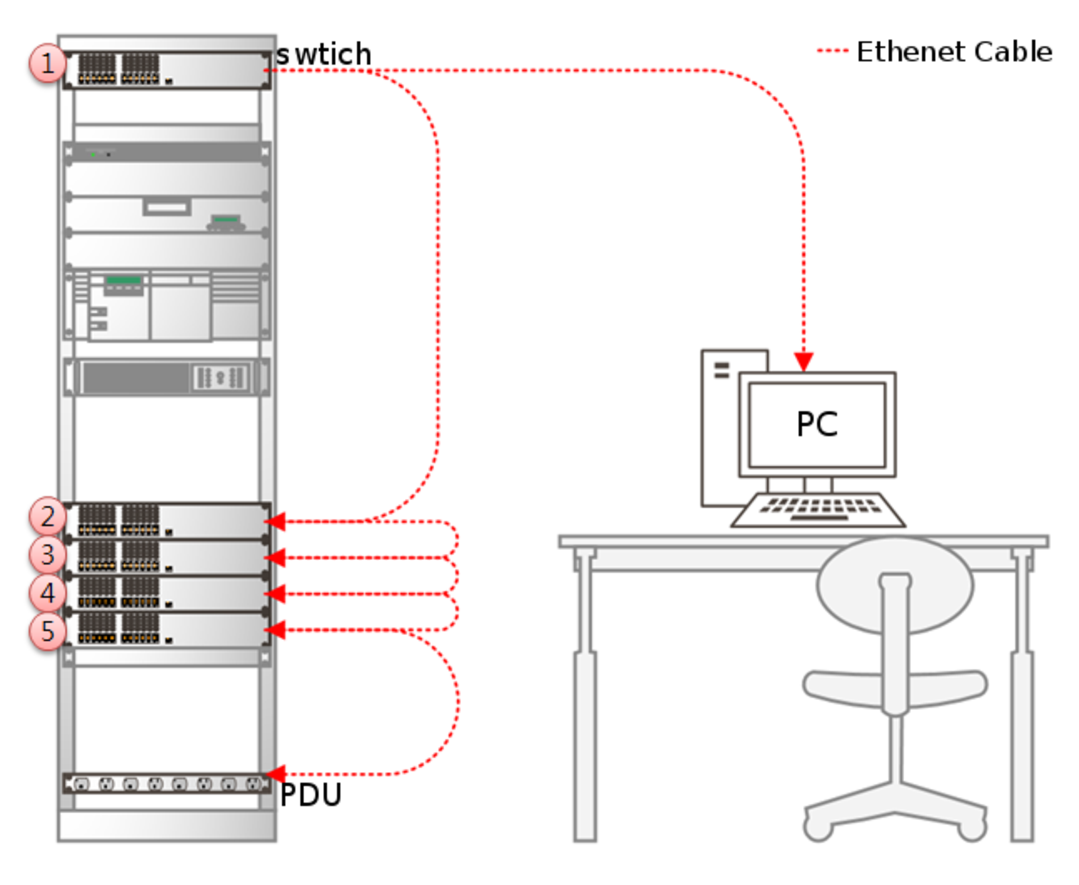
\includegraphics[width=0.6\textwidth]{./images/switch5.eps}
  \caption{테스트 배치}
  \label{fig:switch}   
\end{figure}

이렇게 측정된 응답시간의 mean값은 ASCII 파일로 저장이 되고, 이 ASCII 파일은 그림 \ref{fig:time_table}와 같이 데이터 테이블로 재구성된다. 이렇게 만들어진 데이터 테이블을 이용해 통계 계산과 그래픽을 위한 프로그래밍 언어이자 소프트웨어 환경인 R\citep{r}을 통해 통계적 예측과 분석을 수행한다. 

\begin{figure}[!htb]
  \centering
  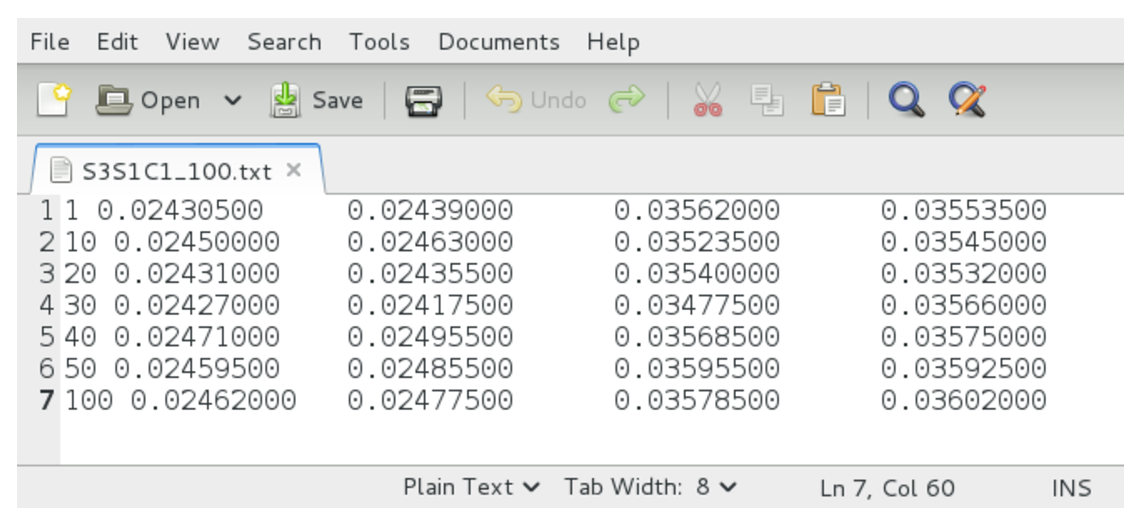
\includegraphics[width=0.8\textwidth]{./images/timetable.eps}
  \caption{데이터 테이블}
  \label{fig:time_table}   
\end{figure}

\clearpage
\section{실험 결과}
\subsection{3.3.1 케이블 길이와 응답시간의 관계}
본 실험에서는 통계적 분석에 앞서 케이블 길이가 길어질수록 응답시간이 클 것이라는 가설을 세웠고, 두 변수 간의 관련성이 연구할 만한 자료인지 판단하기 위해 산점도와 linear fitting을 통한 linear그래프를 그려 변수들의 상관관계를 확인하였다. 그림 \ref{fig:linear}은 스위치의 개수와 SNMP 버전 별로 케이블 길이와 응답시간의 관계를 보여준다. 대부분의 그래프에서 케이블의 길이가 길어질수록 응답시간이 것을 알 수 있다.

\begin{figure}[!htb]
  \centering
  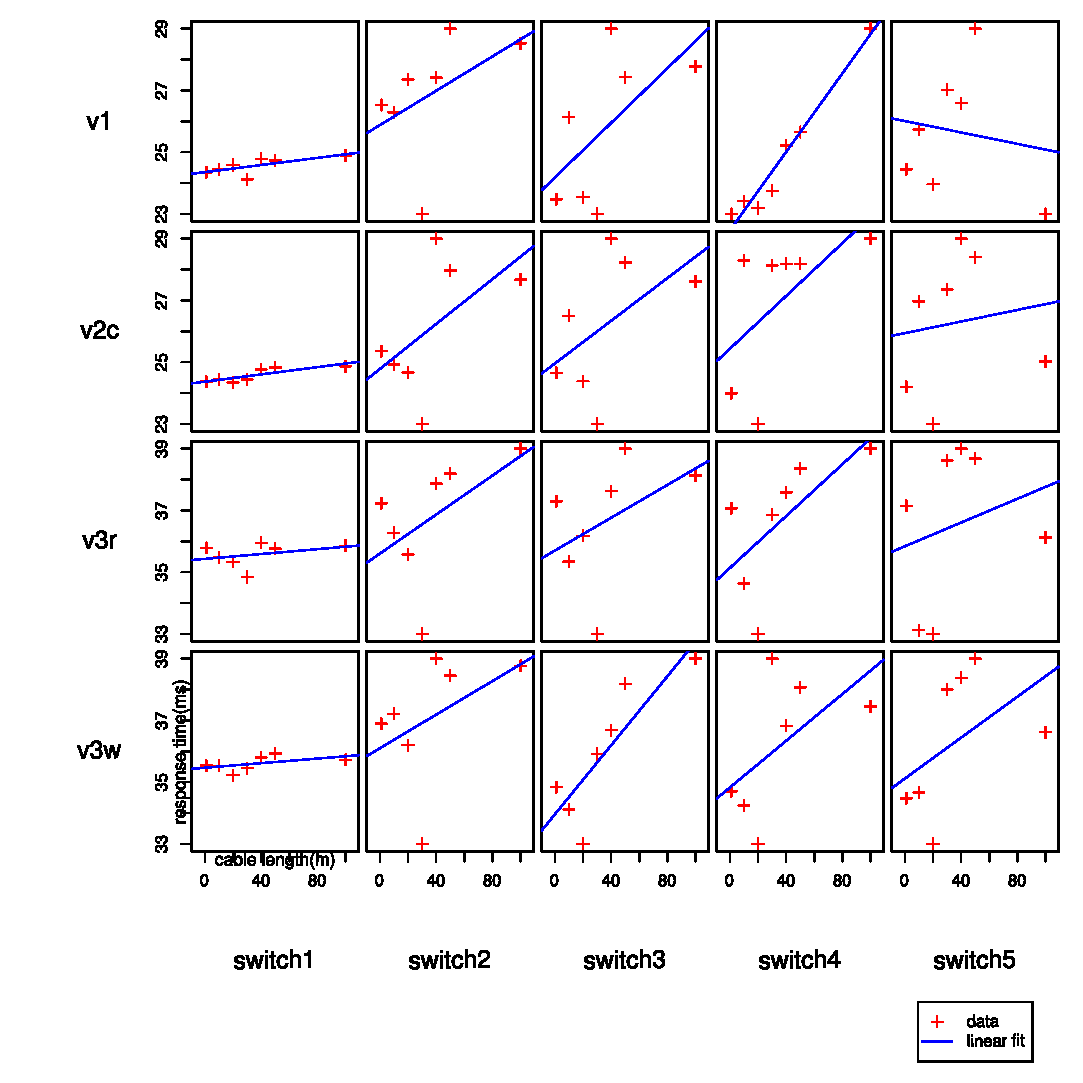
\includegraphics[width=0.9\textwidth]{./images/sleep1_switch.eps}
  \caption{산점도와 linear 그래프}
  \label{fig:linear}   
\end{figure}

\clearpage

\subsection{3.3.2 R을 통한 데이터 분석 및 예측}
본 실험은 데이터 분석에 하나 또는 그 이상의 독립변수(x)의 종속변수(y)에 대한 영향의 추정을 할 수 있는 통계기법인 회귀분석을 사용하였다\citep{analysis}. 회귀분석은 최소 하나 이상의 독립변수의 값에 근거하여 종속변수의 값을 예측하거나 독립변수가 종속변수에 미치는 영향력의 크기를 설명하는데 유용하다. 회귀분석에서 독립변수는 다른 변수에 영향을 미치는 변수이고, 종속변수는 독립변수에 의해 영향을 받는 변수이다. 따라서 독립변수는 케이블 길이이고, 종속변수는 응답시간이다. 종속변수가 독립변수에 어떻게 관련되어 있는가를 나타내는 방정식은 회귀모델이며, 실험의 회귀모델은 식\ref{eq:eps}과 같다. 
\begin{equation} \label{eq:eps}
  y=\alpha + \beta x 
\end{equation}

그림 \ref{fig:s3s1}은 스위치를 세 개 연결하고, Sleep을 1초 걸었을 때 SNMPv2c와 v3w의 단순회귀분석그래프이다. 

\begin{figure}[!htb]
  \centering
  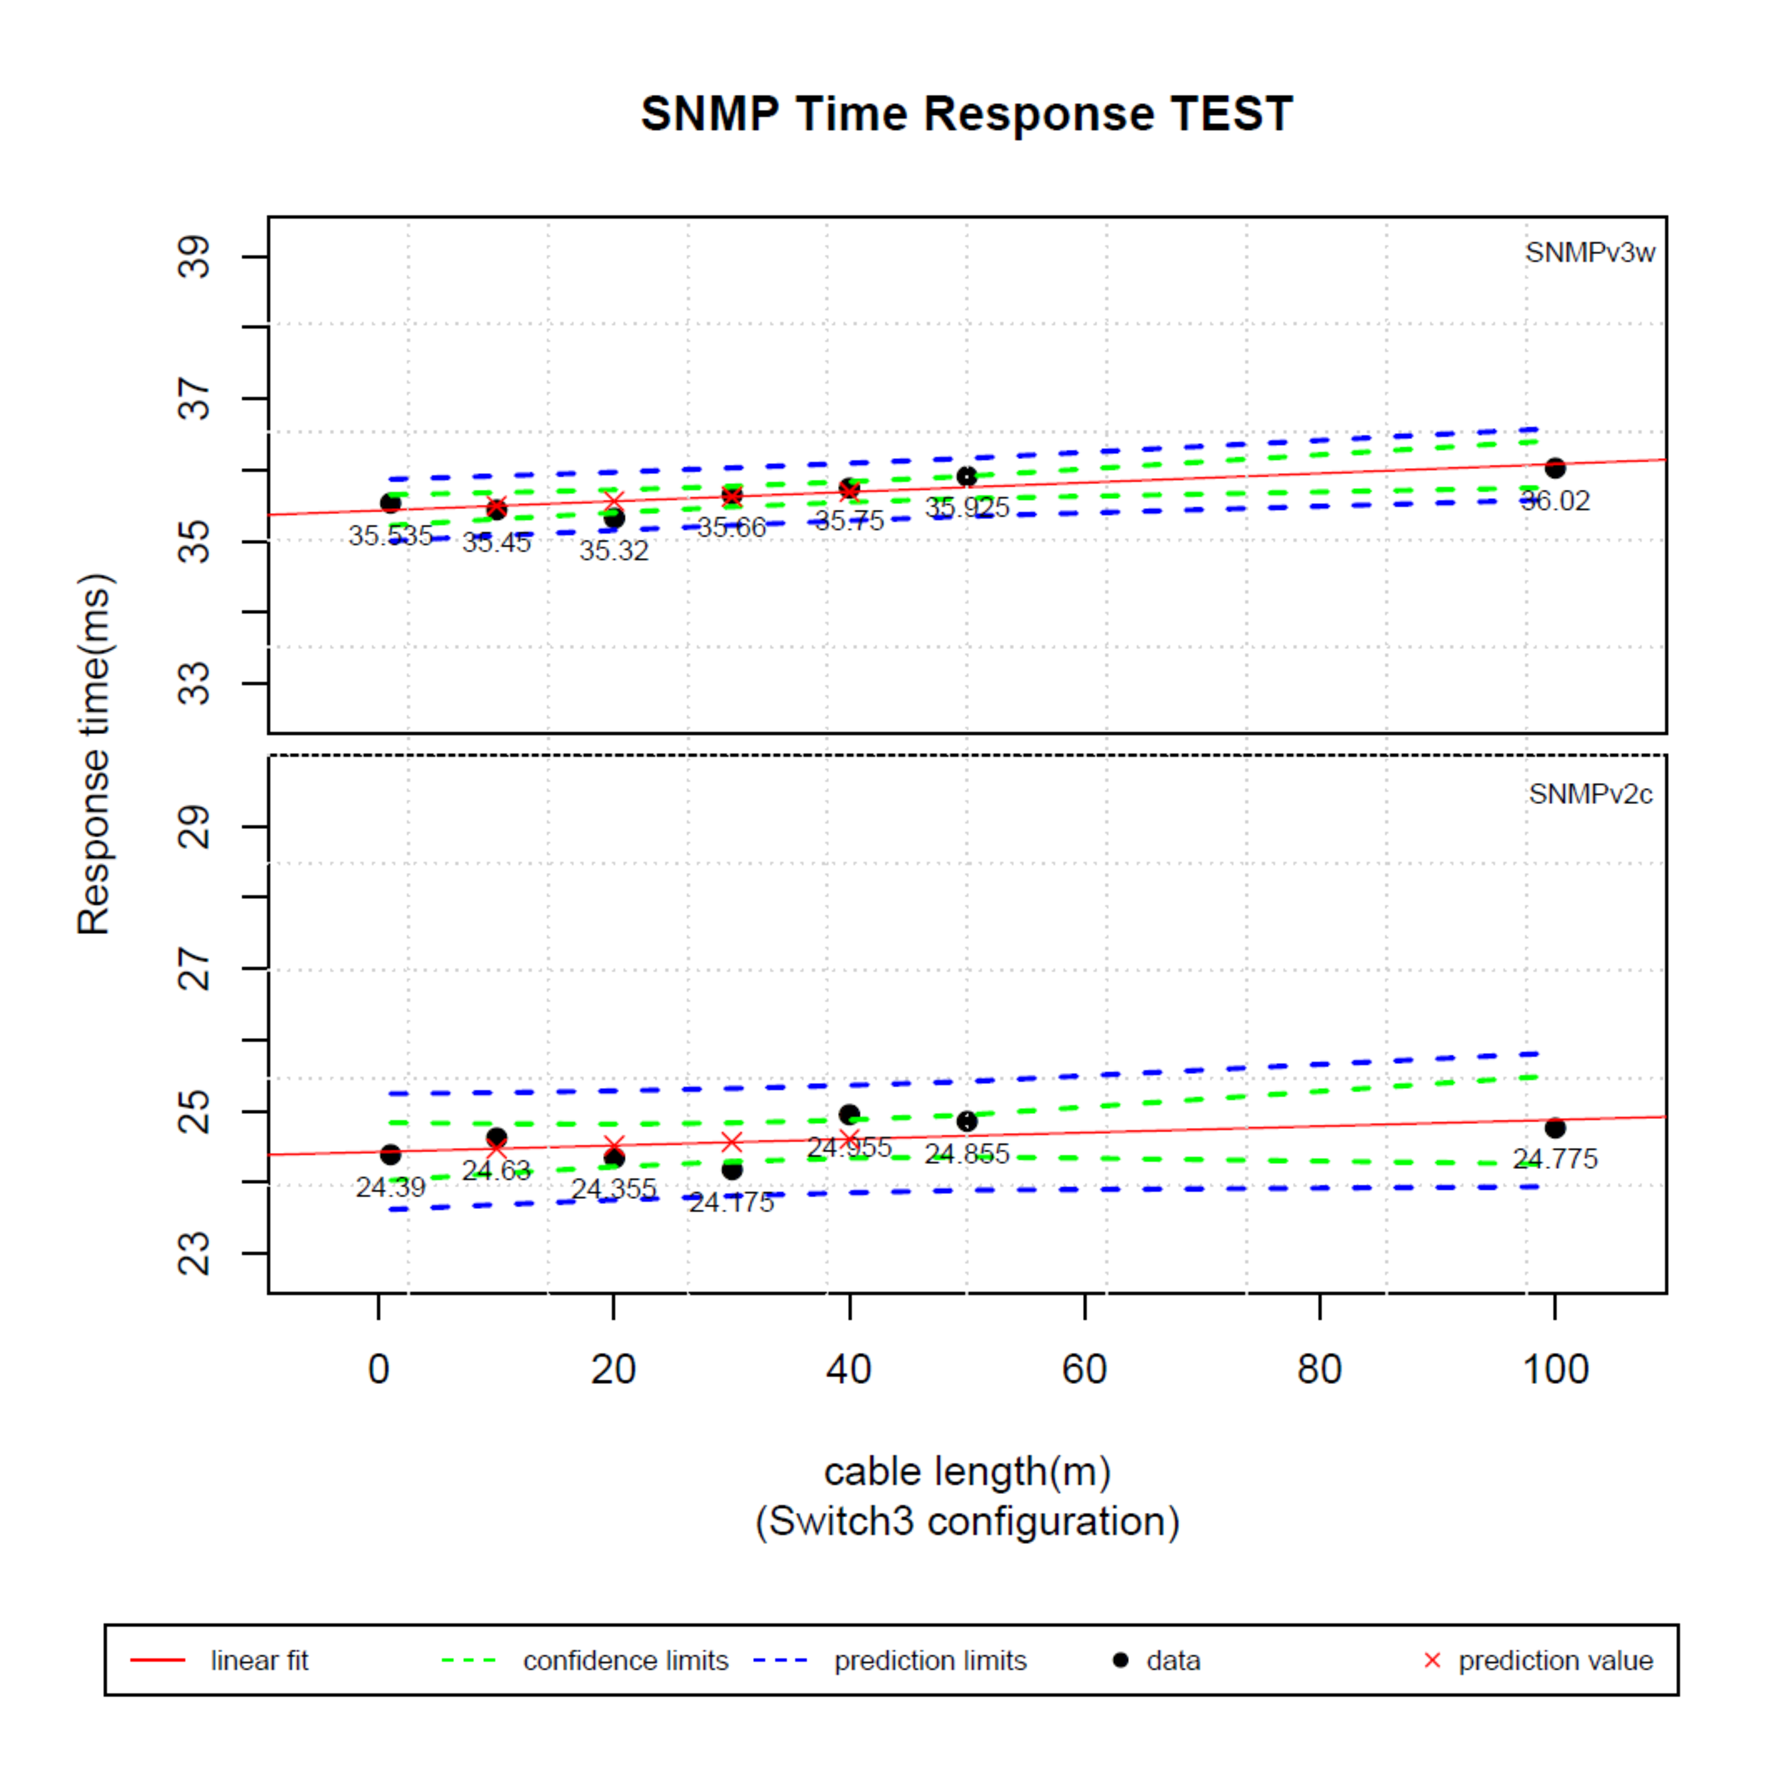
\includegraphics[width=0.88\textwidth]{./images/s3s1.eps}
  \caption{회귀분석 그래프(스위치 3개/Sleep1)}
  \label{fig:s3s1}   
\end{figure}

이 그래프에서 confidence limit(녹색점선)은 추가적인 실험 진행 시 1, 10, 20, 30, 40, 50, 100m의 케이블 길이에서 나올 수 있는 응답시간의 범위를 나타내고, prediction limit(청색점선)은 실험에 사용된 케이블 길이가 아닌 길이의 케이블을 사용하여 응답시간 측정 시에 나올 수 있는 응답시간의 범위이다. ●는 1, 10, 20, 30, 40, 50, 100m의 케이블 길이에서 측정한 결과 값이며, ▲는 1, 50, 100m 길이로 측정한 결과 값으로 linear fitting 피팅을 통해 10, 20, 30, 40m의 길이에서 응답시간을 예측한 값이다. 

\begin{table}[!htb]
\begin{center}
\begin{tabular}{c|c|c|c|c}\hline
길이(m) & 10 & 20 & 30 & 40 \\ \hline
예측응답시간(ms)& 35.50 & 35.56 & 35.63 & 35.69 \\ \hline
실제응답시간(ms)& 35.45 & 35.32 & 35.75 & 36.02 \\ \hline
\end{tabular}
\caption{케이블 길이에 따른 응답시간의 예측과 측정(v3w)}
  \label{table:predict_time}  
\end{center}
\end{table} 
표 \ref{table:predict_time}은 그림 \ref{fig:s3s1}에서 v3w부분을 표식화한 것으로, 이를 참조하면 예측된 응답시간과 실제 측정한 응답시간이 오차범위 내에 있는 것을 확인 할 수 있다.
 
 \subsection{3.3.3 회귀분석 결과와 가설 검증}
 실험 전 세운 가설의 타당성을 입증하기 위하여 회귀분석을 수행하였고 표 \ref{table:regression}는 그 결과이다.
 
\begin{table}[!htb]
\begin{center}
\begin{tabular}{c|c}\hline
Independent variable & Value  \\ \hline\hline
p-value &  0.0155\\ 
F-value &  13\\ 
$  R^2  $ &  0.722\\ 
$ Adjusted R^2 $ & 0.666 \\ \hline
\multicolumn{2}{l}{*p < 0.05} \\ \hline\hline
\end{tabular}
\caption{회귀분석결과(v3w)}
  \label{table:regression}  
\end{center}
\end{table} 
회귀분석에서 $  R^2  $은 종속변수의 총 변동에서 독립변수의 변동에 의해 설명되는 부분이 차지하는 비중을 의미한다. 스위치가 3개 연결 되었을 때, v3w의 경우 응답시간 변동의 약 72.2\%를 케이블 길이 변동에 의해 설명할 수 있다. 또한, p-value가 0.0155로 α인 0.05보다 작으므로 앞서 세운 가설이 통계적으로 유의하다고 할 수 있다. 하지만 대부분의 실험의 결과에서 가설이 통계적으로 유의하지 않았다\ref{cha:result}. 이는 측정한 시간이 오차범위 내에 있지만 분석에 사용된 샘플링의 수가 적고, 실험 시 케이블의 길이, 하드웨어 자체의 속도 등의 환경이 완벽하게 동일하지 않아 정밀한 실험이 진행되지 않았음에서 이유를 찾을 수 있다. 

\clearpage
\appendix
\addappheadtotoc
\renewcommand*\printchaptername{\Large\bfseries\appendixname~}
\chapter{회귀분석 그래프}

\section{Switch 1}
 \begin{figure}[!htb]
  \centering
  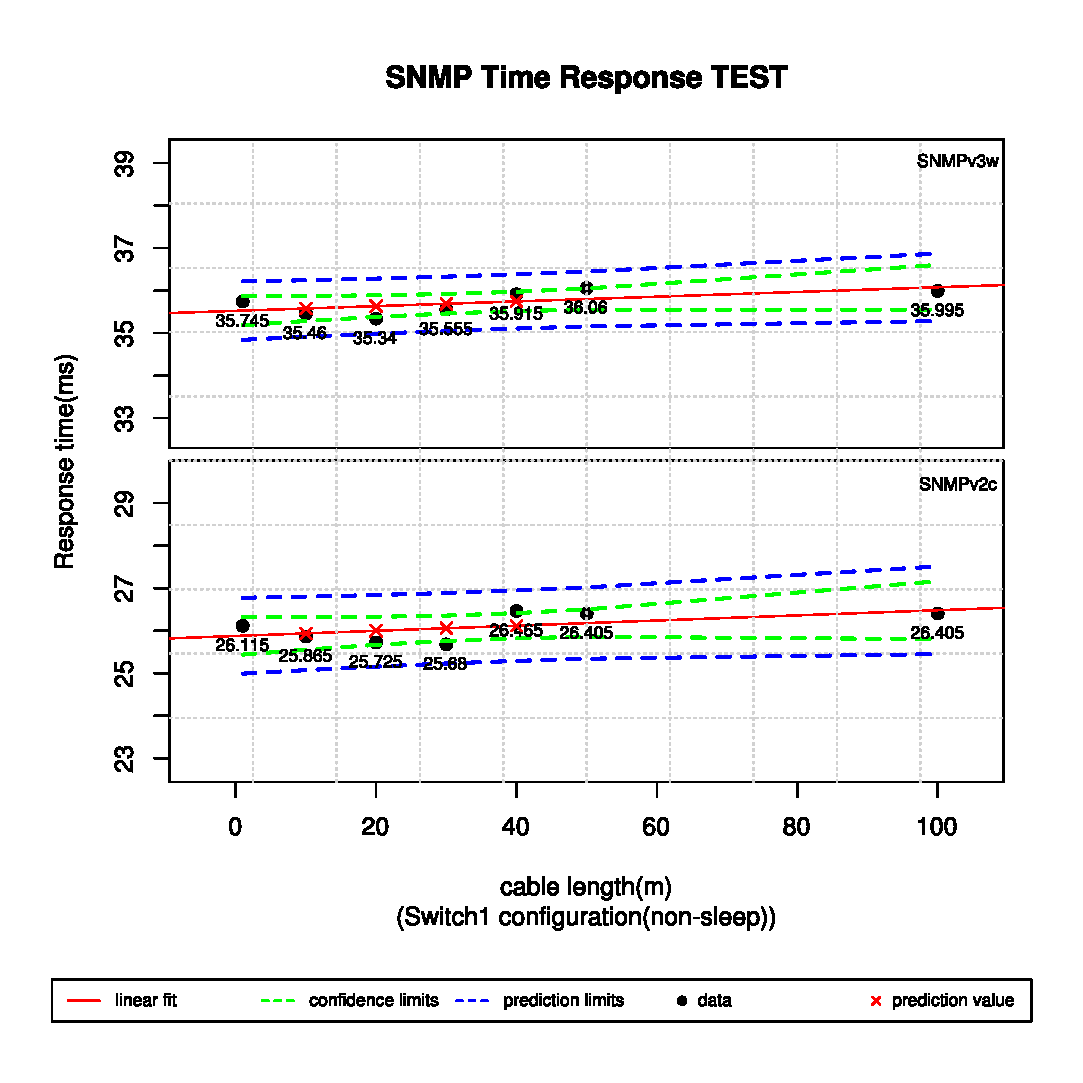
\includegraphics[width=0.55\textwidth]{./images/s1sx.eps}
  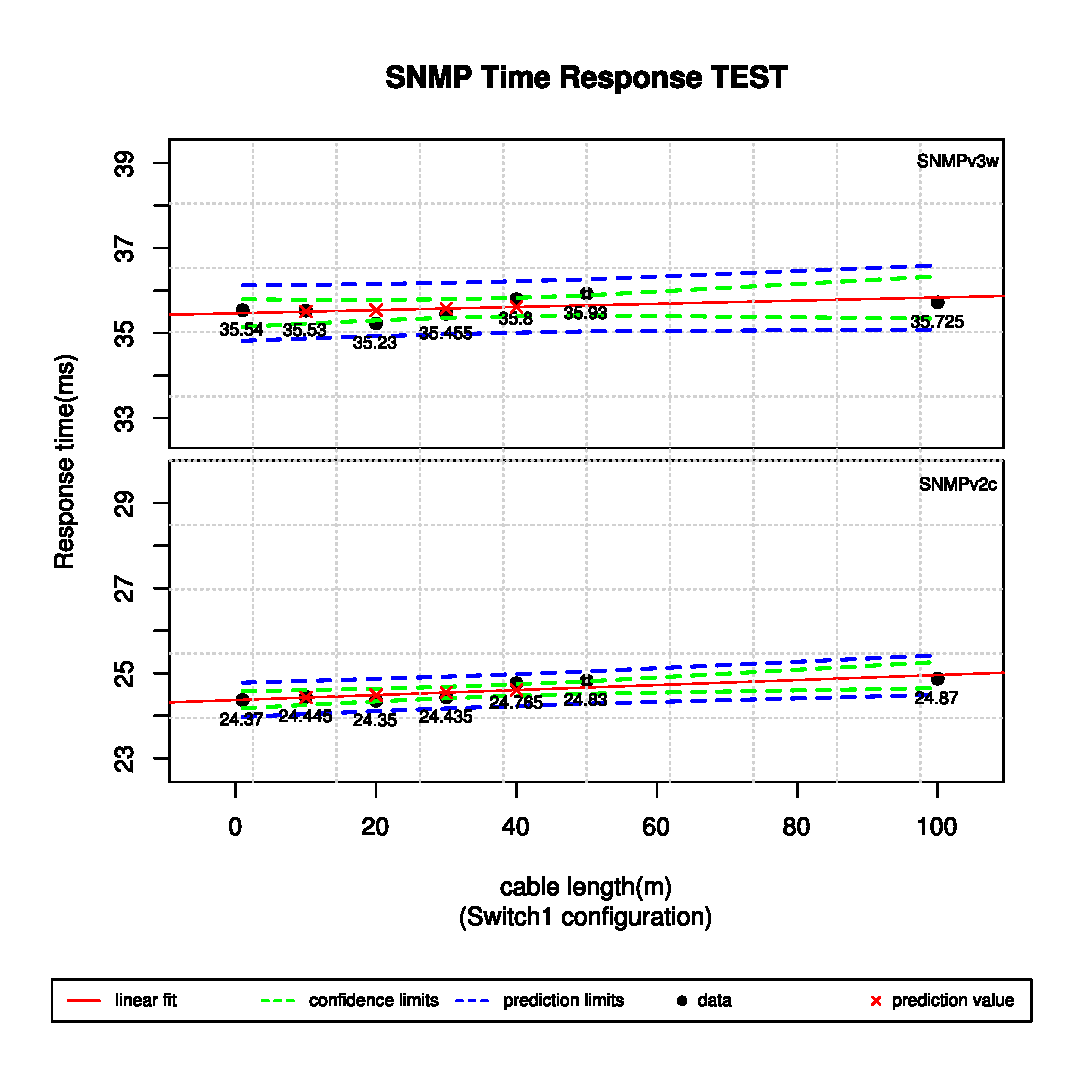
\includegraphics[width=0.55\textwidth]{./images/s1s1.eps}
  \caption{Swtich1 configuration}
\end{figure}
\clearpage

\section{Switch 2}
 \begin{figure}[!htb]
  \centering
  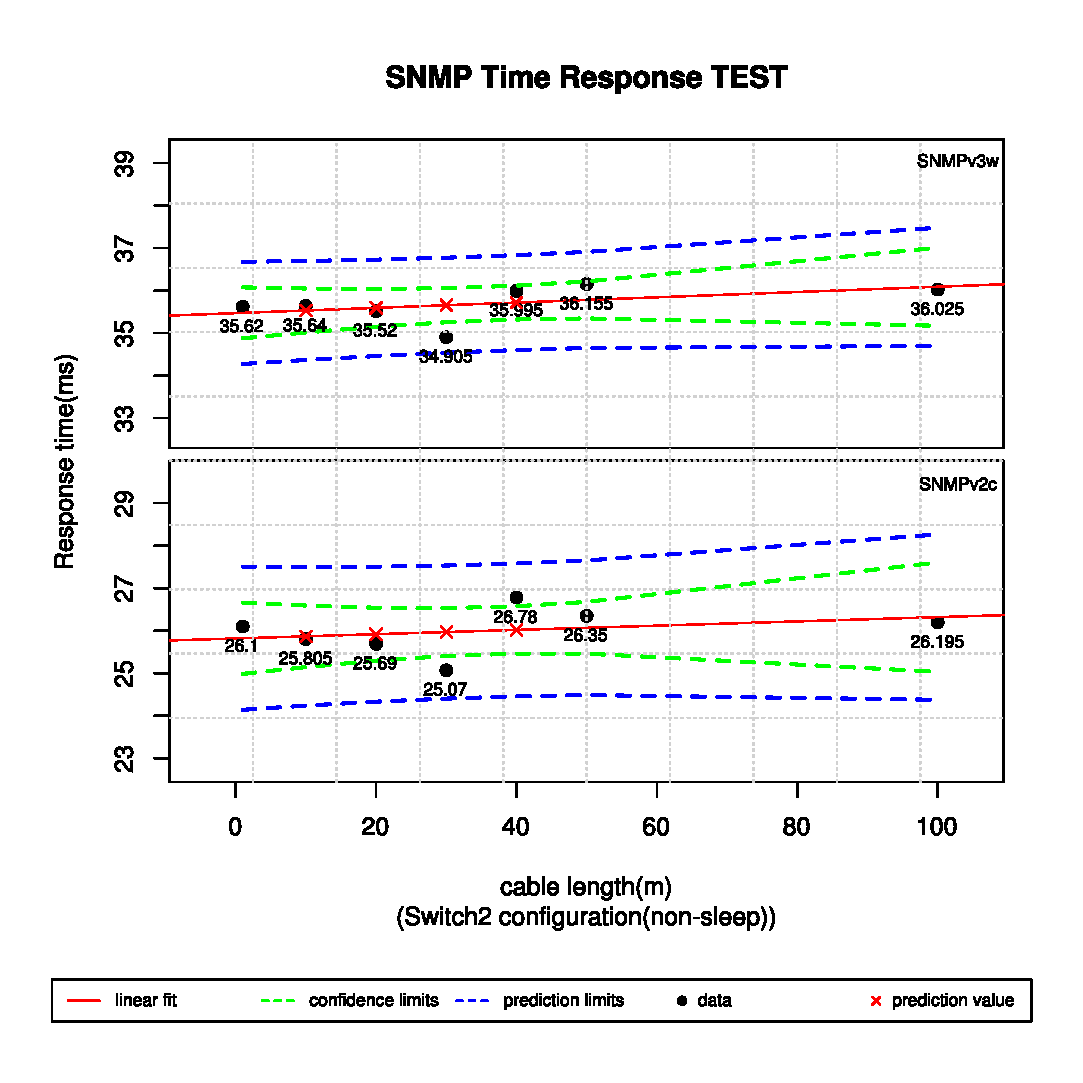
\includegraphics[width=0.55\textwidth]{./images/s2sx.eps}
  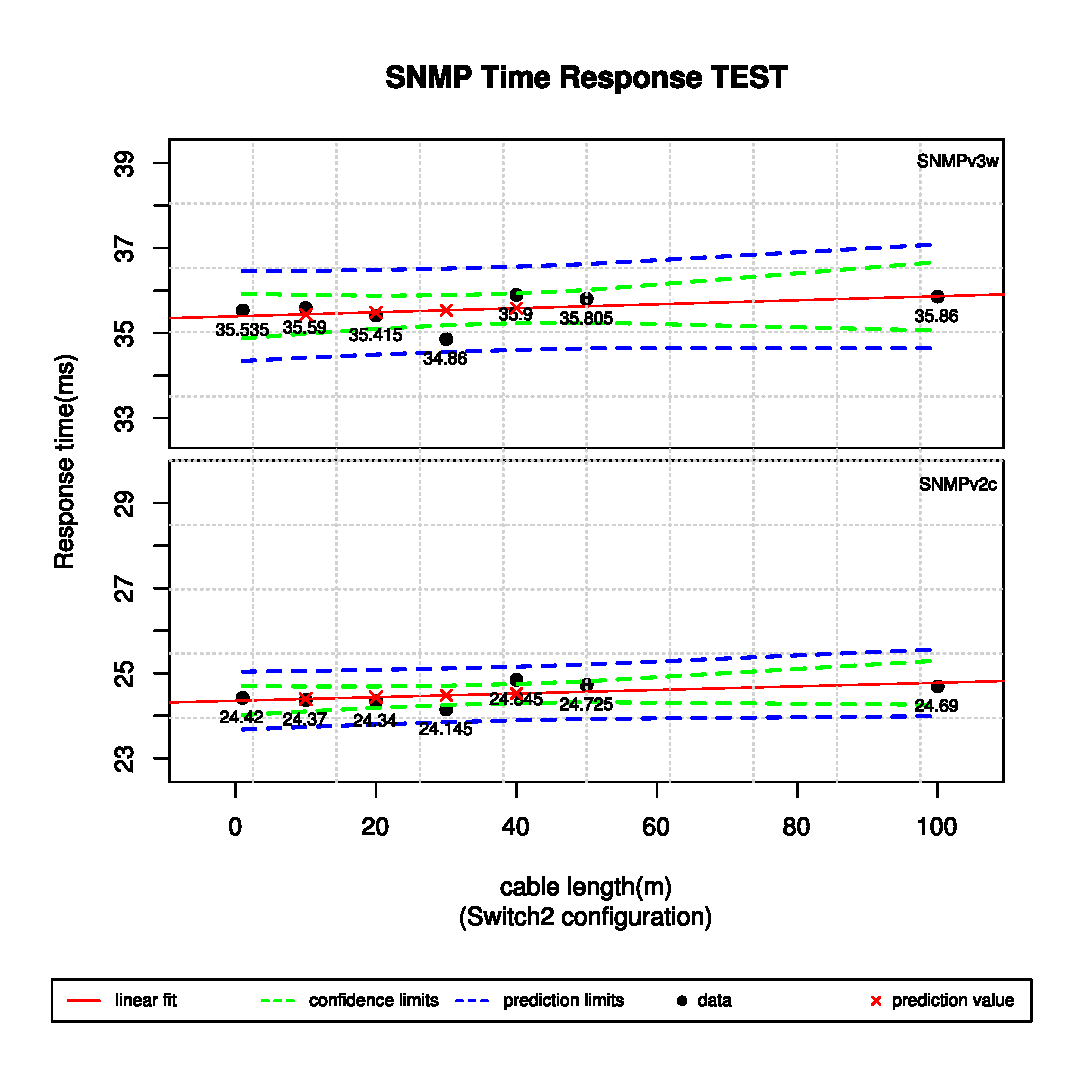
\includegraphics[width=0.55\textwidth]{./images/s2s1.eps}
  \caption{Swtich2 configuration}
\end{figure}
\clearpage

\section{Switch 3}
 \begin{figure}[!htb]
  \centering
  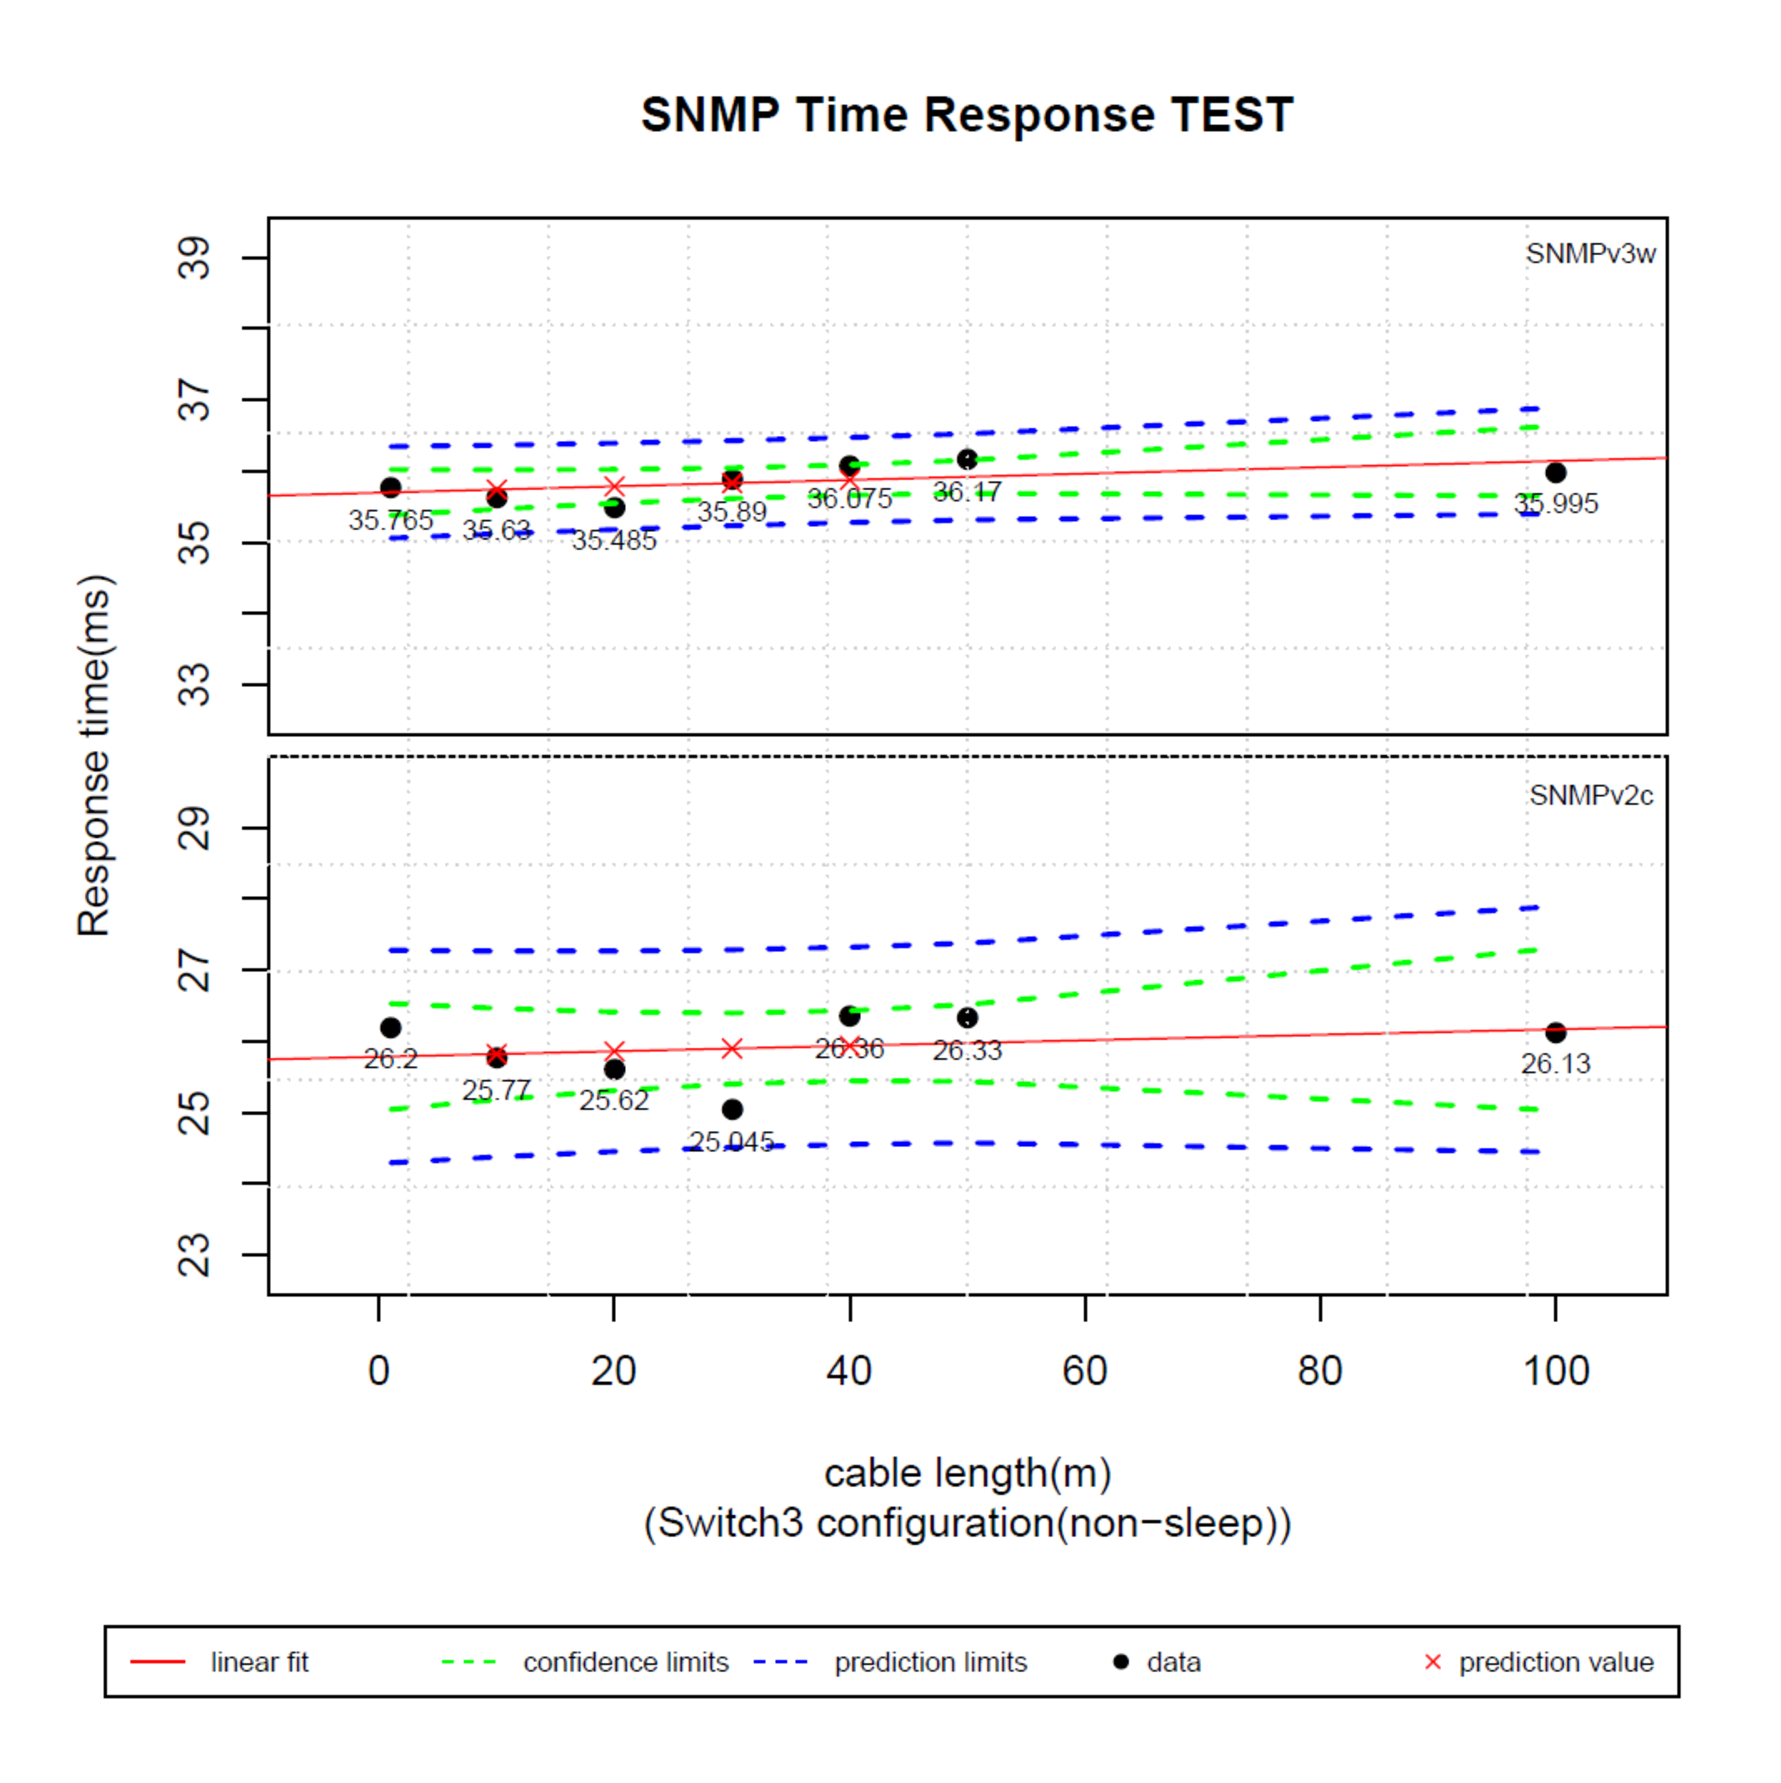
\includegraphics[width=0.55\textwidth]{./images/s3sx.eps}
  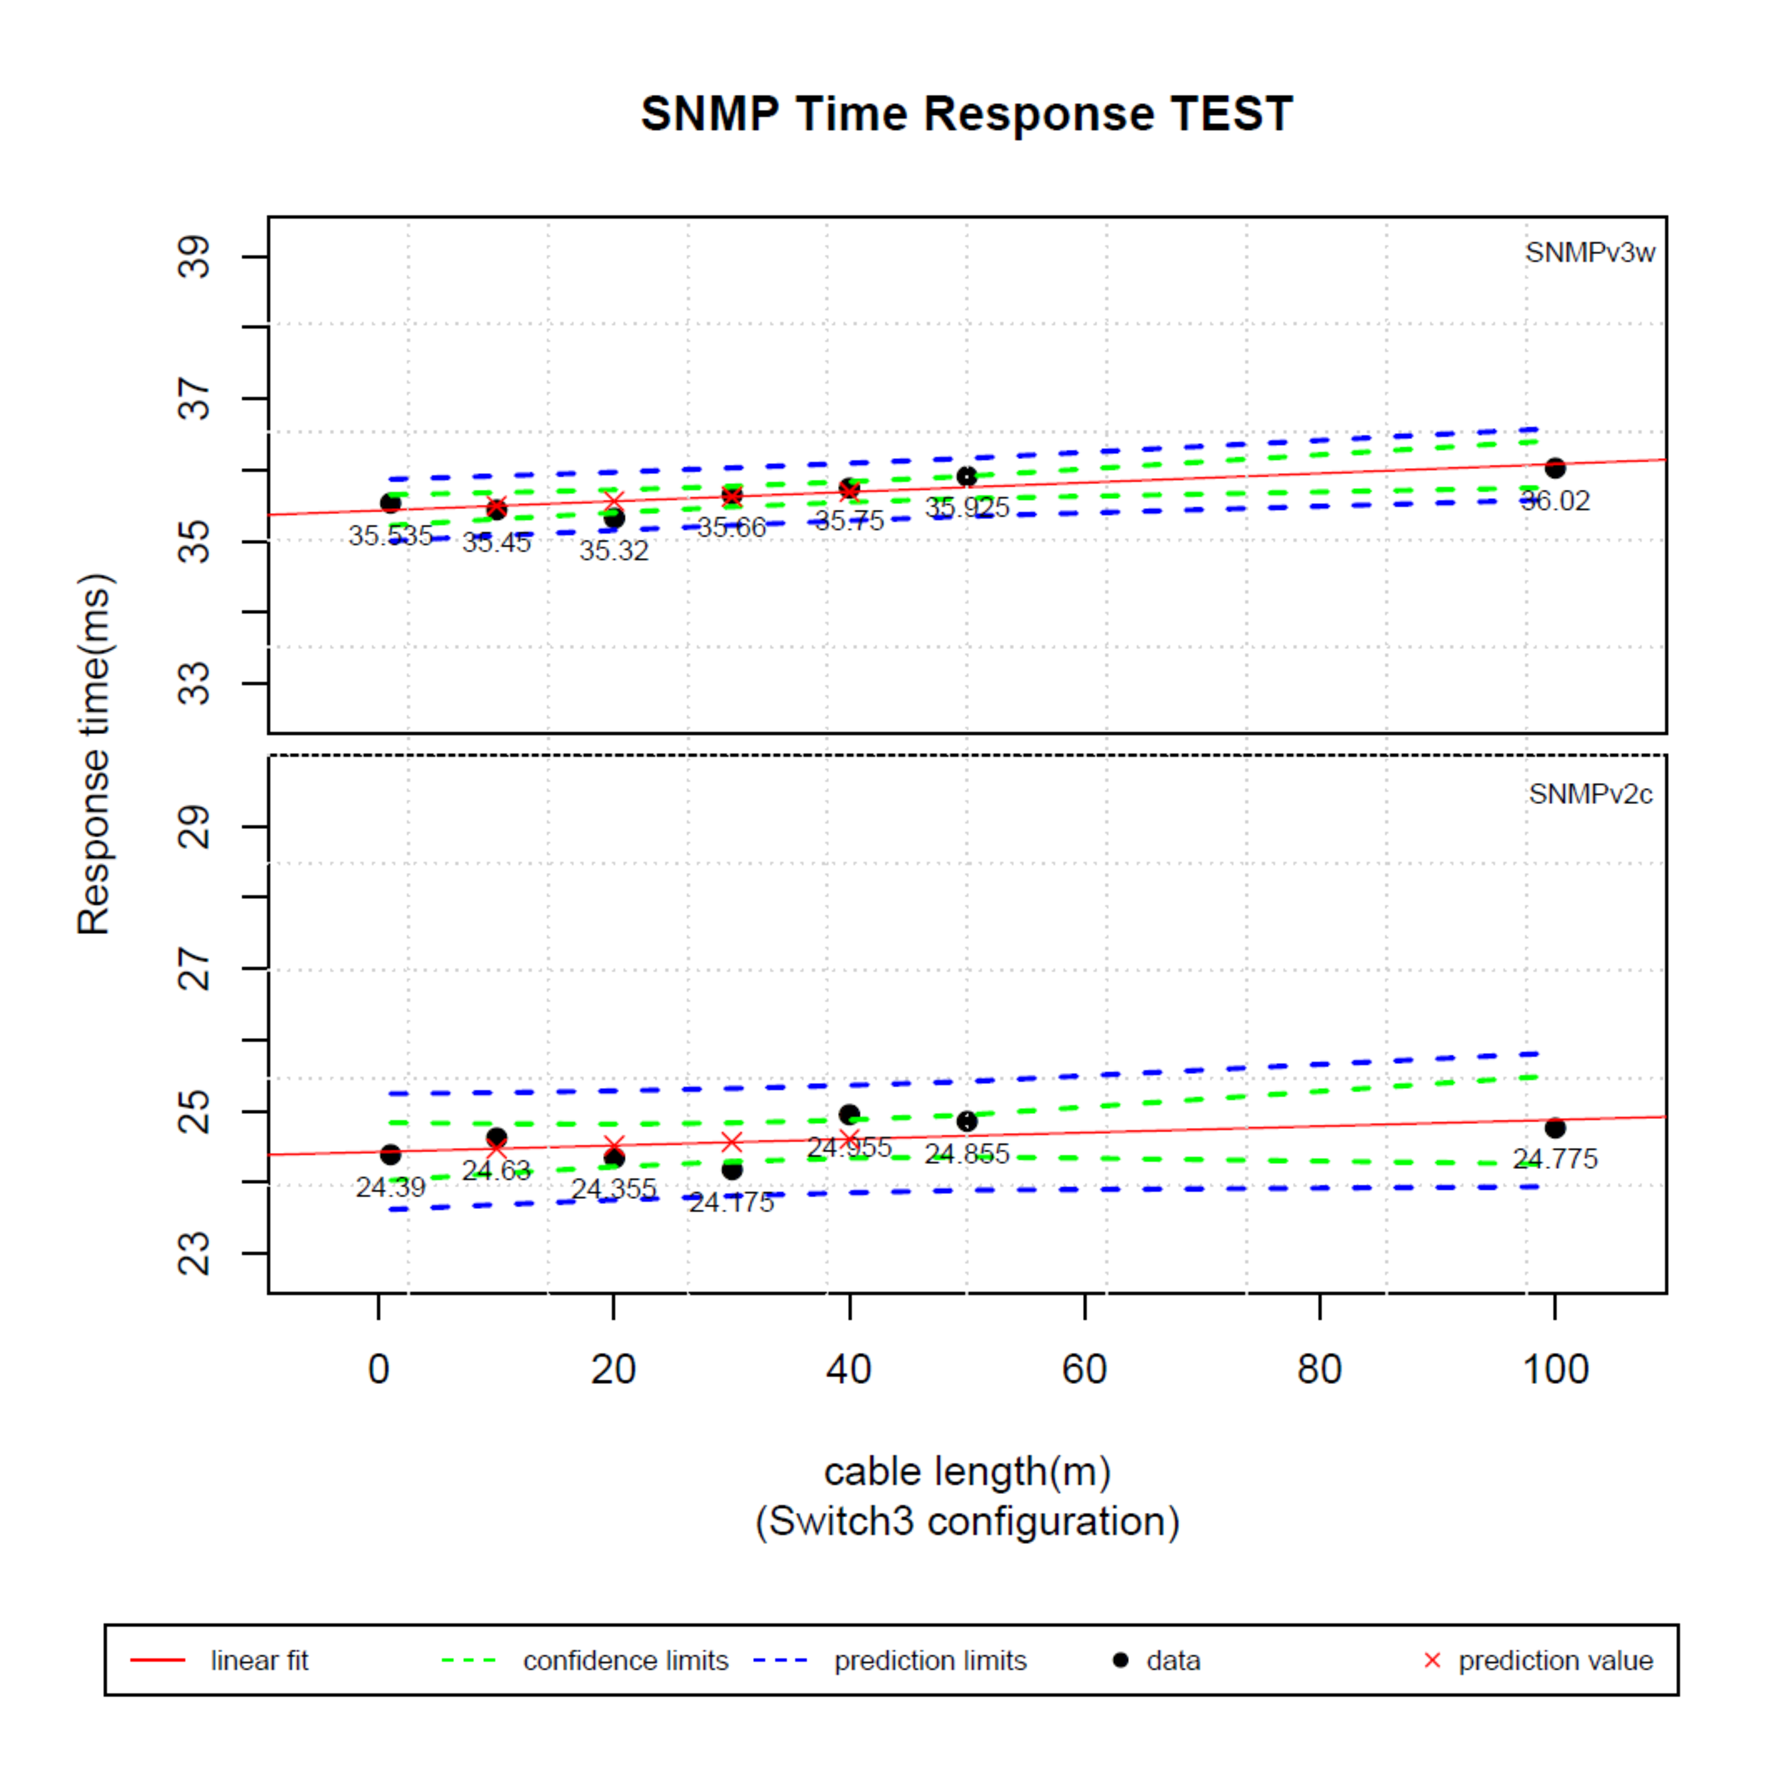
\includegraphics[width=0.55\textwidth]{./images/s3s1.eps}
  \caption{Swtich3 configuration}
\end{figure}
\clearpage

\section{Switch 4}
 \begin{figure}[!htb]
  \centering
  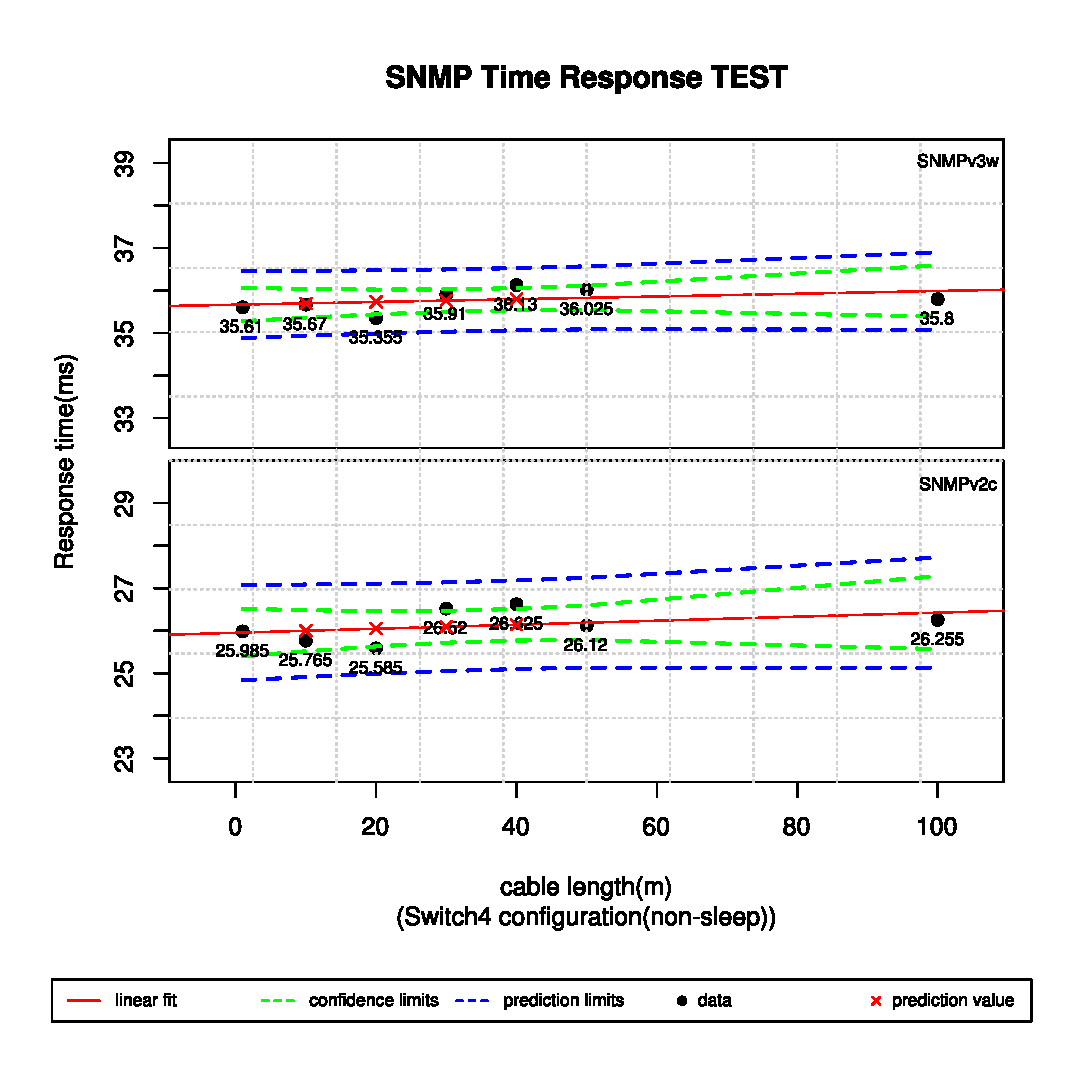
\includegraphics[width=0.55\textwidth]{./images/s4sx.eps}
  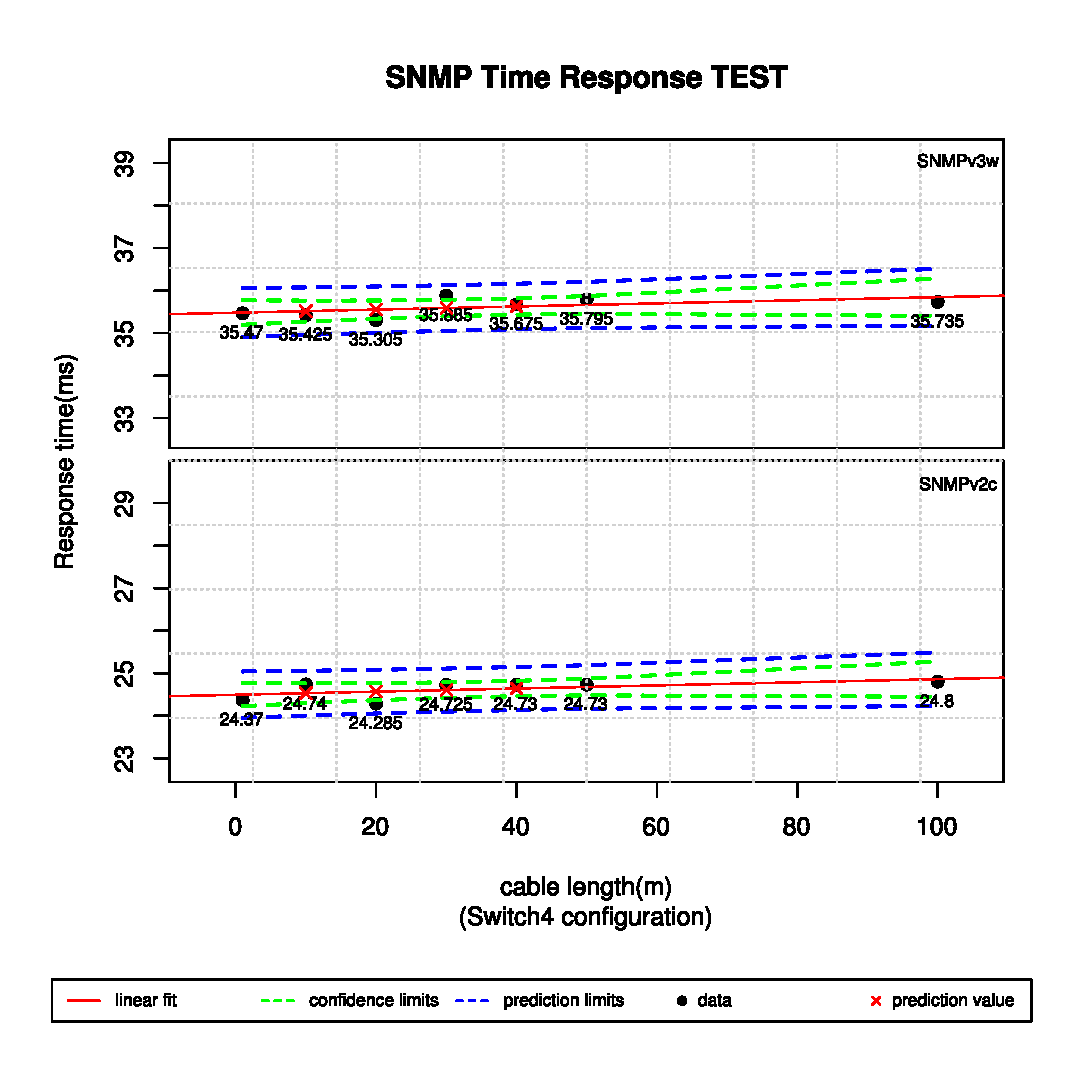
\includegraphics[width=0.55\textwidth]{./images/s4s1.eps}
  \caption{Swtich4 configuration}
\end{figure}
\clearpage

\section{Switch 5}
 \begin{figure}[!htb]
  \centering
  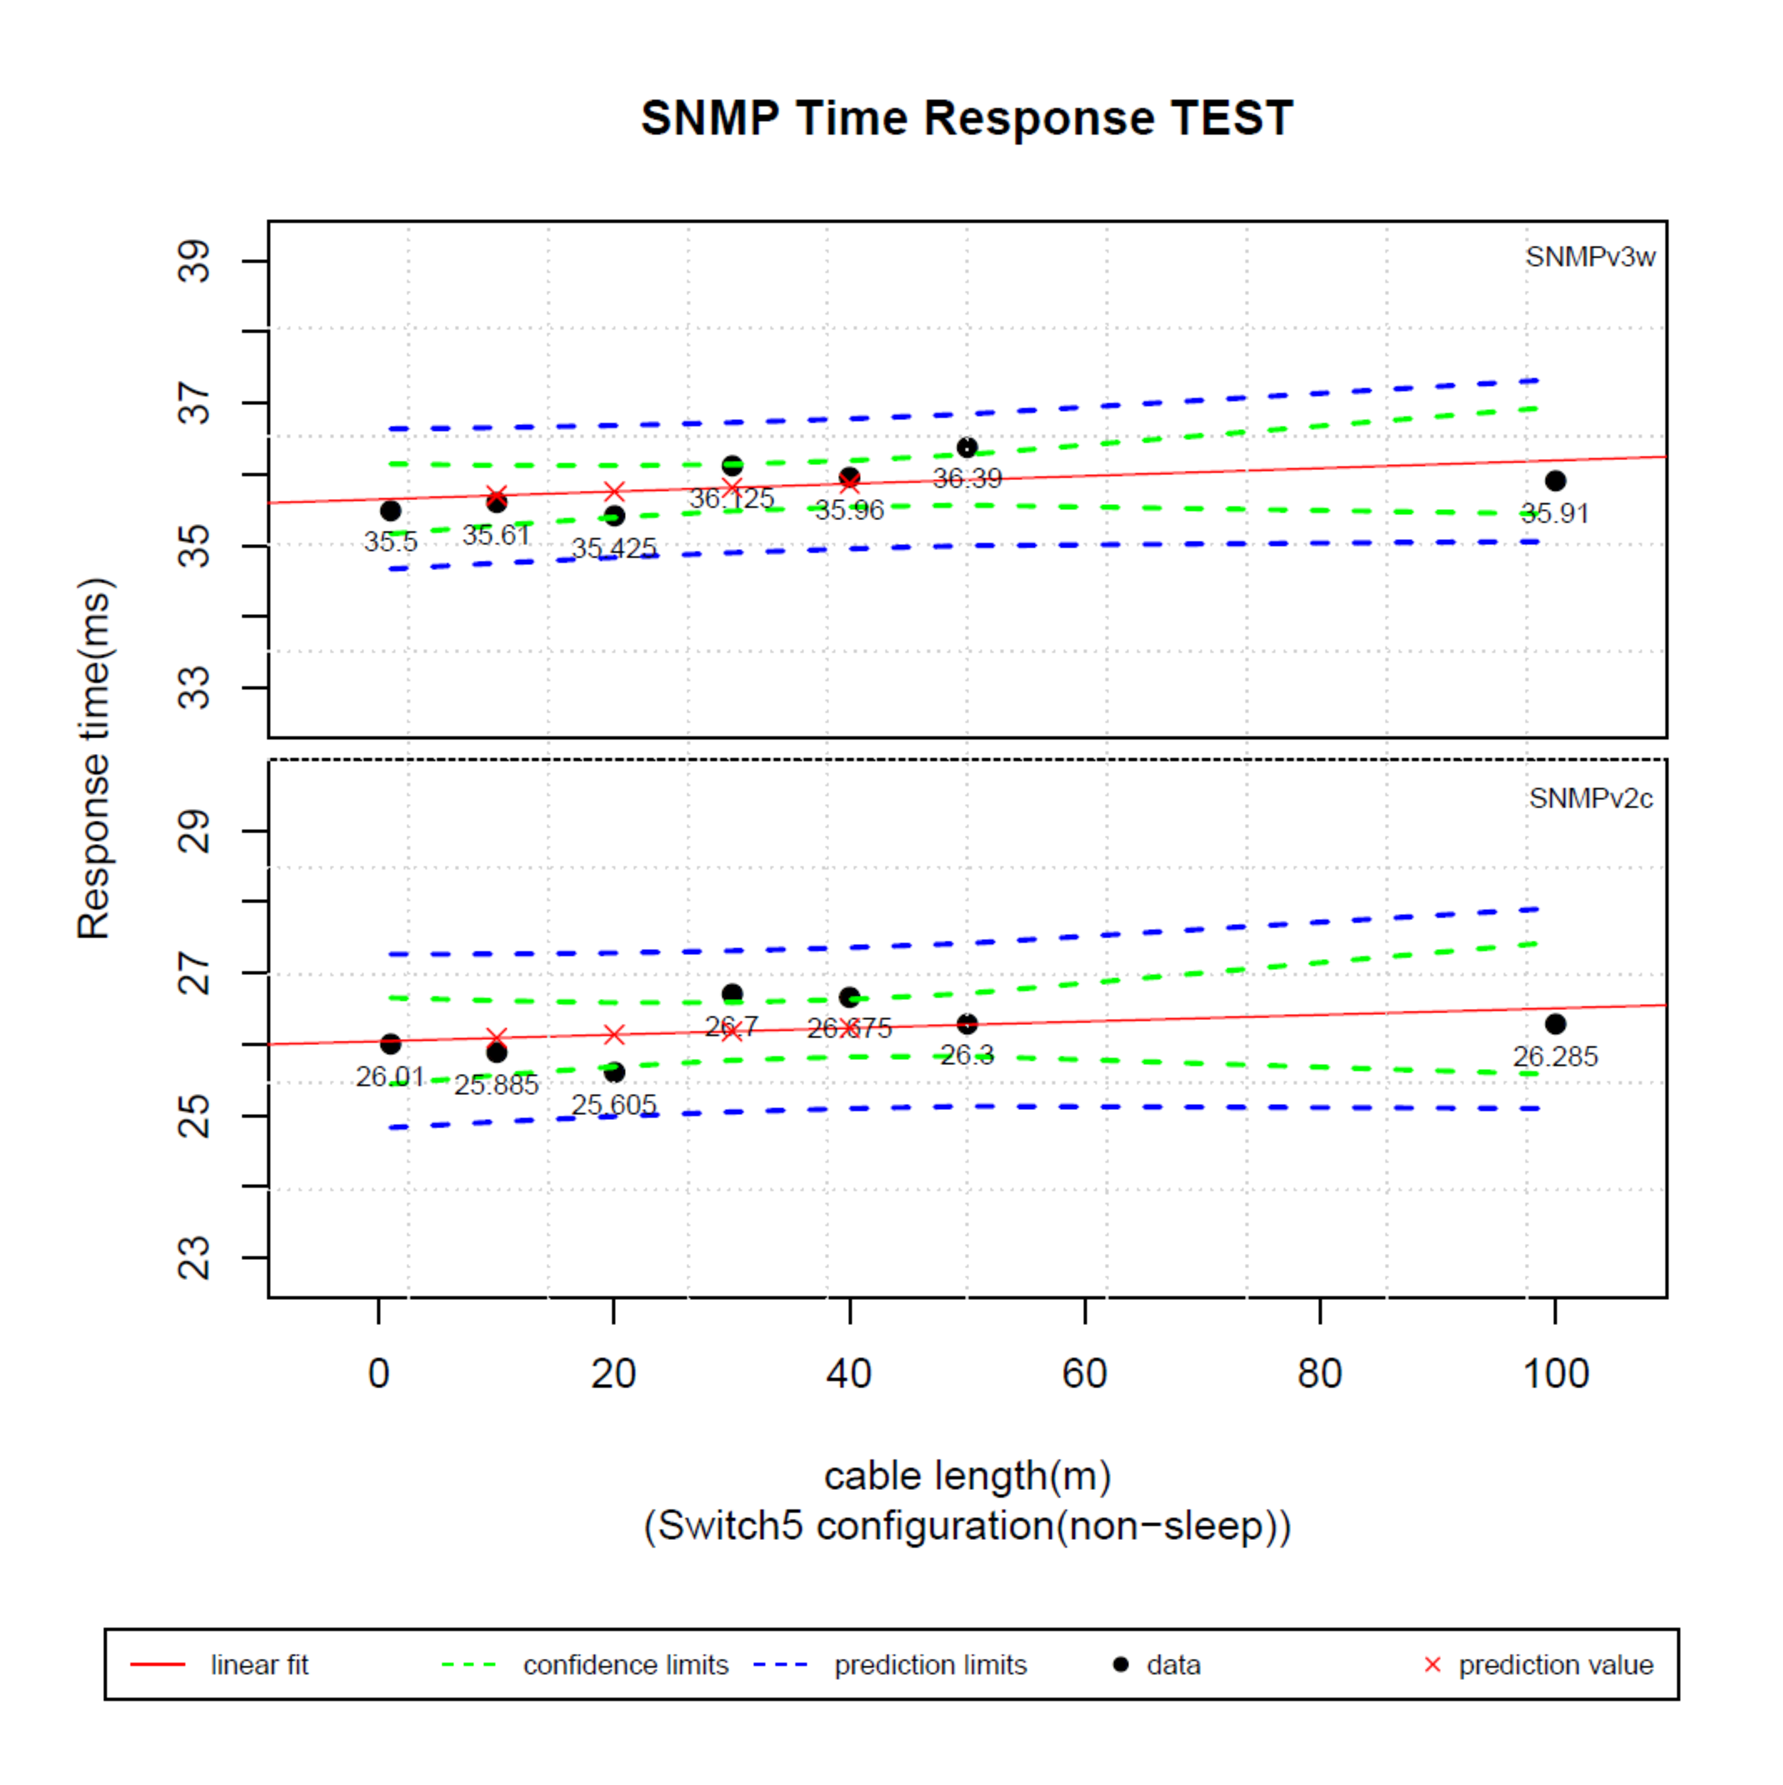
\includegraphics[width=0.55\textwidth]{./images/s5sx.eps}
  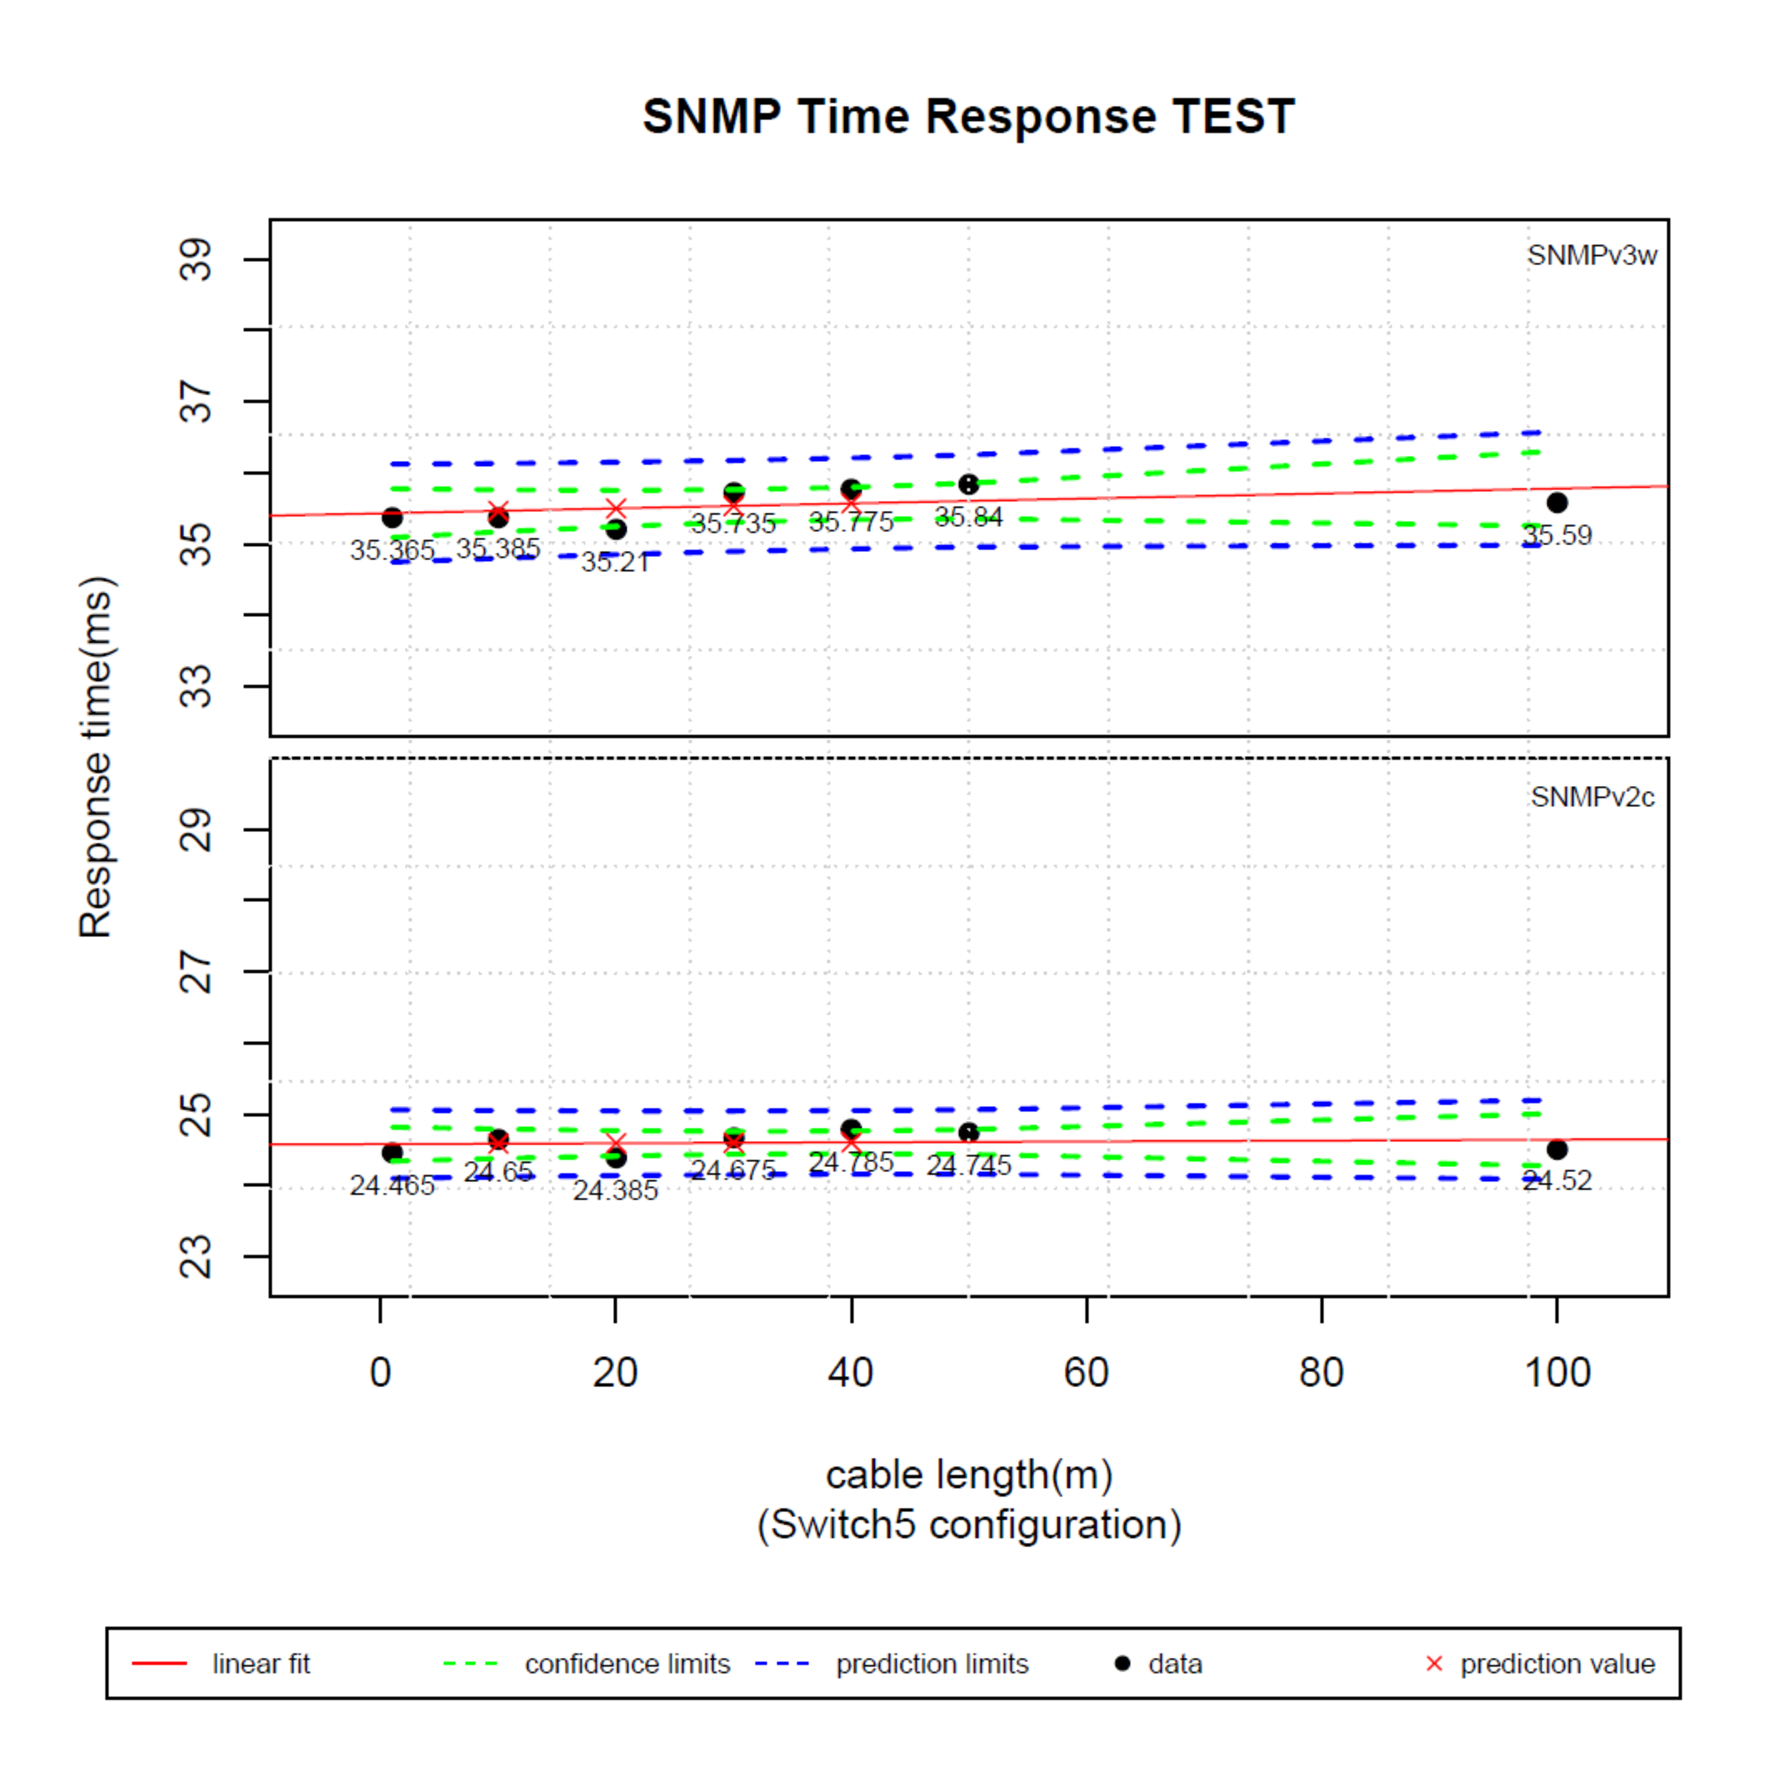
\includegraphics[width=0.55\textwidth]{./images/s5s1.eps}
  \caption{Swtich4 configuration} 
\end{figure}

\chapter{회귀분석 결과}\label{cha:result}
\section{Switch 1}

\begin{table}[h!]
\begin{center}
\begin{tabular}{c|c||c||c||c}
\multicolumn{5}{c}{Switch1/Sleepx}\\ \hline\hline
\multicolumn{1}{c|}{}& \multicolumn{4}{c}{Value}\\
\cline{1-5}
Independent variable & v1 & v2c & v3r & v3w      \\ \hline\hline
p-value &  0.164 &  0.166 & 0.105  &  0.111\\ 
F-value &  2.65 &  2.63&  3.9 &  3.73\\ 
$  R^2  $ &  0.347  &  0.344&  0.438 &  0.427\\ 
Adjusted $  R^2  $ & 0.0216 & 0.213 & 0.326 & 0.313\\ \hline\hline
\multicolumn{5}{r}{*p < 0.05} \\
\multicolumn{5}{c}{Switch1/Sleep1}\\ \hline\hline
\multicolumn{1}{c|}{}& \multicolumn{4}{c}{Value}\\
\cline{1-5}
Independent variable & v1 & v2c & v3r & v3w     \\ \hline\hline
p-value &  0.0802 &  0.0176& 0.464 &  0.231\\ 
F-value &  4.79  &  12.1&  0.628 &  1.86\\ 
$  R^2  $ &  0.489 &  0.708 &  0.112  &  0.271\\ 
Adjusted $  R^2  $ & 0.387 & 0.65 & -0.0661 & 0.125\\ \hline\hline
\multicolumn{5}{r}{*p < 0.05} 
\end{tabular}
\caption{Switch1 Regression Analysis Result }
\end{center}
\end{table} 
\clearpage

\section{Switch 2}
\begin{table}[h!]
\begin{center}
\begin{tabular}{c|c||c||c||c}
\multicolumn{5}{c}{Switch2/Sleepx}\\ \hline\hline
\multicolumn{1}{c|}{}& \multicolumn{4}{c}{Value}\\
\cline{1-5}
Independent variable & v1 & v2c & v3r & v3w      \\ \hline\hline
p-value & 0.293 & 0.508 & 0.263 & 0.272\\ 
F-value & 1.38 & 0.507 & 1.59 & 1.52\\ 
$  R^2  $ & 0.217 & 0.092 & 0.242 & 0.233\\ 
Adjusted $  R^2  $ & 0.0598 & -0.0896 & 0.09 & 0.0799\\ \hline\hline
\multicolumn{5}{r}{*p < 0.05} \\ 
\multicolumn{5}{c}{Switch2/Sleep1}\\ \hline\hline
\multicolumn{1}{c|}{}& \multicolumn{4}{c}{Value}\\
\cline{1-5}
Independent variable & v1 & v2c & v3r & v3w      \\ \hline\hline
p-value &  0.294 &  0.179& 0.235  &  0.335\\ 
F-value &  1.38 &  2.22 &  1.82  &  1.14\\ 
$  R^2  $ &  0.216 &  0.307&  0.267 & 0.185\\ 
Adjusted $  R^2  $ & 0.059 & 0.169 & 0.121 & 0.0224\\ \hline\hline
\multicolumn{5}{r}{*p < 0.05} \\ 
\end{tabular}
\caption{Switch1 Regression Analysis Result }
\end{center}
\end{table} 
\clearpage

\section{Switch 3}
\begin{table}[h!]
\begin{center}
\begin{tabular}{c|c||c||c||c}
\multicolumn{5}{c}{Switch3/Sleepx}\\ \hline\hline
\multicolumn{1}{c|}{}& \multicolumn{4}{c}{Value}\\
\cline{1-5}
Independent variable & v1 & v2c & v3r & v3w      \\ \hline\hline
p-value & 0.336 & 0.563 & 0.115 & 0.158\\ 
F-value & 1.13  & 0.383 & 3.62 & 2.75\\ 
$  R^2  $ & 0.184 & 0.0711 & 0.42 & 0.355\\ 
Adjusted $  R^2  $ & 0.0211 & -0.115 & 0.304 & 0.225\\ \hline\hline
\multicolumn{5}{r}{*p < 0.05} \\ 
\multicolumn{5}{c}{Switch3/Sleep1}\\ \hline\hline
\multicolumn{1}{c|}{}& \multicolumn{4}{c}{Value}\\
\cline{1-5}
Independent variable & v1 & v2c & v3r & v3w      \\ \hline\hline
p-value & 0.154 & 0.243 & 0.33 & 0.0155\\ 
F-value & 2.82 & 1.75 & 1.16 & 13\\ 
$  R^2  $ & 0.361 & 0.259 & 0.189 & 0.722\\ 
Adjusted $  R^2  $ & 0.233  & 0.111& 0.0262 & 0.666\\ \hline\hline
\multicolumn{5}{r}{*p < 0.05} \\ 
\end{tabular}
\caption{Switch3 Regression Analysis Result }
\end{center}
\end{table} 
\clearpage

\section{Switch 4}
\begin{table}[h!]
\begin{center}
\begin{tabular}{c|c||c||c||c}
\multicolumn{5}{c}{Switch4/Sleepx}\\ \hline\hline
\multicolumn{1}{c|}{}& \multicolumn{4}{c}{Value}\\
\cline{1-5}
Independent variable & v1 & v2c & v3r & v3w      \\ \hline\hline
p-value &  0.409 & 0.36 & 0.419 & 0.374\\ 
F-value &  0.813 & 1.01 & 0.775 & 0.954\\ 
$  R^2  $ & 0.14 & 0.169 & 0.134 & 0.16\\ 
Adjusted $  R^2  $ & -0.0322 & 0.00245 & -0.039 & -0.00774\\ \hline\hline
\multicolumn{5}{r}{*p < 0.05} \\
\multicolumn{5}{c}{Switch4/Sleep1}\\ \hline\hline
\multicolumn{1}{c|}{}& \multicolumn{4}{c}{Value}\\
\cline{1-5}
Independent variable & v1 & v2c & v3r & v3w      \\ \hline\hline
p-value & 0.000107 & 0.168 & 0.112 & 0.19\\ 
F-value & 122 &  2.59&  3.7  &  2.3\\ 
$  R^2  $ & 0.961 & 0.342& 0.426 & 0.315\\ 
Adjusted $  R^2  $ & 0.953 & 0.21& 0.311 & 0.178\\ \hline\hline
\multicolumn{5}{r}{*p < 0.05} \\ 
\end{tabular}
\caption{Switch4 Regression Analysis Result }
\end{center}
\end{table} 
\clearpage

\section{Switch 5}
\begin{table}[h!]
\begin{center}
\begin{tabular}{c|c||c||c||c}
\multicolumn{5}{c}{Switch5/Sleepx}\\ \hline\hline
\multicolumn{1}{c|}{}& \multicolumn{4}{c}{Value}\\
\cline{1-5}
Independent variable & v1 & v2c & v3r & v3w      \\ \hline\hline
p-value & 0.616 & 0.405& 0.159 & 0.242\\ 
F-value & 0.285 & 0.828& 2.74 & 1.76\\ 
$  R^2  $ & 0.054 & 0.142& 0.354 & 0.26\\ 
Adjusted $  R^2  $ & -0.135 & -0.0295& 0.224 & 0.112\\ \hline\hline
\multicolumn{5}{r}{*p < 0.05} \\ 
\multicolumn{5}{c}{Switch5/Sleep1}\\ \hline\hline
\multicolumn{1}{c|}{}& \multicolumn{4}{c}{Value}\\
\cline{1-5}
Independent variable & v1 & v2c & v3r & v3w      \\ \hline\hline
p-value & 0.751 & 0.768 & 0.595 & 0.28\\ 
F-value & 0.113 & 0.0968 & 0.323 & 1.47\\ 
$  R^2  $ & 0.022 & 0.01 9& 0.0606 & 0.227\\ 
Adjusted $  R^2  $ & -0.174 & -0.177 & -0.127 & 0.072\\ \hline\hline
\multicolumn{5}{r}{*p < 0.05} \\ 
\end{tabular}
\caption{Switch1 Regression Analysis Result }
\end{center}
\end{table} 






\clearpage
\bibliographystyle{unsrtnat}
\bibliography{./refs}

\end{document}

